% arara: bibtex
% arara: pdflatex
% arara: pdflatex
\documentclass[12pt,journal]{IEEEtran}			
\usepackage{	array,
			booktabs,
			cite,
			enumitem,
			epstopdf,
			fancyhdr,
			graphicx,
			lipsum,
			lscape,
			mathtools,
			mcode,
			nomencl,			
			parallel,
			rotating,
			soul,
			wrapfig,
			}
\usepackage{soul}
\usepackage[final]{pdfpages}
\usepackage{mcode}
\graphicspath{ {./images/} } % Graphics Path
\bibliographystyle{plain}
\usepackage{listings}
\usepackage{amsmath}

%-------------------------------------
%              ARDUINO
%-------------------------------------

% Arduino style for highlighting
\newcommand\arduinostyle{\lstset{%
    language=C++,
    %otherkeywords={dac,Serial,},
    basicstyle=\footnotesize,% basic font setting
    frame=tb,                         % Any extra options here
    showstringspaces=false            % 
}}

% Arduino Enviornment
\lstnewenvironment{arduino}[1][]
{
\arduinostyle
\lstset{#1}
}
{}

% Arduino for external files
\newcommand\arduinoexternal[2][]{{
\arduinostyle
\lstinputlisting[#1]{#2}}}

% Arduino for inline
\newcommand\arduinoinline[1]{{\arduinostyle\lstinline!#1!}}

\usepackage[utf8]{inputenc}

% Default fixed font does not support bold face
\DeclareFixedFont{\ttb}{T1}{txtt}{bx}{n}{10} % for bold
\DeclareFixedFont{\ttm}{T1}{txtt}{m}{n}{10}  % for normal

% Custom colors
\usepackage{color}
\definecolor{deepblue}{rgb}{0,0,0.5}
\definecolor{deepred}{rgb}{0.6,0,0}
\definecolor{deepgreen}{rgb}{0,0.5,0}

%-------------------------------------
%             PYTHON
%-------------------------------------

% Python style for highlighting
\newcommand\pythonstyle{\lstset{
language=Python,
basicstyle=\ttm,
otherkeywords={self},             % Add keywords here
keywordstyle=\ttb\color{deepblue},
emph={MyClass,__init__,GUI,SerialPort,Error,DataError,ImageError,},          % Custom highlighting
emphstyle=\ttb\color{deepred},    % Custom highlighting style
stringstyle=\color{deepgreen},
frame=tb,                         % Any extra options here
showstringspaces=false            % 
}}


% Python environment
\lstnewenvironment{python}[1][]
{
\pythonstyle
\lstset{#1}
}
{}

% Python for external files
\newcommand\pythonexternal[2][]{{
\pythonstyle
\lstinputlisting[#1]{#2}}}

% Python for inline
\newcommand\pythoninline[1]{{\pythonstyle\lstinline!#1!}}

\setlength\parindent{0.33in}

%-------------------------------------
%       LTPSICE NETLIST
%-------------------------------------

% LTPSICE NETLIST style for highlighting
\newcommand\ltspicestyle{\lstset{
language=Clean, 
basicstyle=\scriptsize
}}


% LTPSICE NETLIST environment
\lstnewenvironment{ltspice}[1][]
{
\ltspicestyle
\lstset{#1}
}
{}

% LTPSICE NETLIST for external files
\newcommand\ltspiceexternal[2][]{{
\ltspicestyle
\lstinputlisting[#1]{#2}}}


\setlength\parindent{0.33in}

\begin{document}

\title{The Design and Implementation of a Scanning Fabry-Perot Interferometer for Use in Measuring Multiple Modes in Lasers}
\author{David M Houston}

\maketitle

% Project Goals

\begin{abstract}
A scanning mirror Fabry-Perot Interferometer (sFPI) was designed, built, and implemented to measure the modes of a laser beam. It has a finesse of 155 and free spectral range of 3.75 GHz with a resolution bandwidth of 24 MHz. A piezoelectric device will change the spacing of the mirrors, allowing scanning across multiple free spectral ranges. A voltage-source driver provides a controllable signal to a piezoelectric device. The spectral frequency content will be captured by a photodetector and amplified by a transimpedance amplifier. This can be analyzed one of two ways. Either sent to a micro-controller-computer pair which processes, displays, and stores this data locally on a hard disk, or sampled by an oscilloscope which can take the place of the mircocontroller.
\end{abstract}

\begin{IEEEkeywords}
FSR, sFPI, Python
\end{IEEEkeywords}

% Background Section
\section{Introduction} \label{ss:introduction}
The current sFPI (Spectra-Physics SP-470-06) is bulky and requires various appendages in order to operate. It requires a separate photodiode and data collection device (i.e. oscilloscope). This makes it cumbersome to use. The new model has been constructed to reduce the overall real estate and make the operation more user friendly. It has a pre-installed photodiode as well as an integrated application which communicates directly with an onboard microcontroller to process and display the spectral content of the cavity. The application increases the functionality of the device by calibrating the incoming signal based on user input of the free spectral range of the cavity which prompts the application to mathematically scale the output for analysis. While the newly development sFPI seems to be superior to the other it has its disadvantages. The frequency of the driver is only 2.35 Hz, making it much slower than real-time analysis.

\section{Background} \label{ss:background}
In order to understand how the sFPI works, a fundamental principle must be explained. In its static state, a cavity\footnote{Define what a cavity is} can hold a specific number longitudinal modes, proportional to the length of the cavity ($L$). Verheyen's book on laser electronics gives an adequate definition for a cavity mode:
\\
\begin{quote}
A cavity mode is a field distribution that reproduces itself in relative shape and in relative phase after a round trip through the system~\cite{verdeyen}
\end{quote}
\leavevmode \\
\indent Each mode has an order of the form \textit{(m,n,q)}, where \textit{m, n,} and \textit{q} are integers. The transverse modes are represented by \textit{m} and \textit{n}, and the longitudinal modes are represented by \textit{q}. Typically only the $TEM_{0,0,q}$ modes are examined because it makes the math easier, however higher order transverse modes are prevalent in the system. For our purposes we will only be examining the longitudinal modes. However, when the length of the cavity changes ($\Delta L$), so does the orders of the modes which can occupy length $L+\Delta L$. In order to achieve a maximum transmission, $\Delta L$ must be on the order of a wavelength, corresponding to a q+1 increase in the mode order. Any other change in length ($\Delta L$) not on that order will result in little to no transmission of the cavity beam. The separation of the maximum transmission peaks is defined as the free spectral range (FSR) and can be expressed by $\text{FSR}=c/2L$, where \textit{c} is the speed of light in a vacuum. The FSR is described by a frequency, however it can also be related to spacial frequency as well. Figure~\ref{fig:fsr} graphically describes the free spectral range.

Since this is not a perfect cavity, the photon-lifetime is described by an exponential decay rate, $e^{-t/\tau}$. The line shape of the cavity, which has the shape of a lorentzian, is the Fourier transform of the photon-lifetime. The line shape is the transmission intensity of the deviations of frequencies from the fundamental. The full-width at half maximum of the line shape is the bandwidth of the cavity. Typically bandwidth is not expressed, but rather the finesse of the cavity. The finesse is defined as the ratio of the free spectral range to the bandwidth of the cavity (Eq.~\ref{eq:finesse}). 

\begin{equation}
\mathcal{F} = \frac{\pi}{2sin^{-1}(1/\sqrt{F})}
\label{eq:finesse}
\end{equation}

The finesse is related by a factor defined as the coefficient of finesse ($F$) which is proportional to reflectivity of the mirrors used (Eq.~\ref{eq:cof}).

\begin{equation}
F = \frac{4R}{(1-R)^2}
\label{eq:cof}
\end{equation}  

In order to increase the finesse and overall performance of the sFPI cavity, dielectrically coated mirrors with high reflectivity at the principle wavelength are used. The reflectivity of these mirrors is typically $>90\%$. Since the reflectivity is greater than 50\% the simplified Eq.~\ref{eq:finesse_lth_50} can be used to approximate the finesse. This is because at small values of $x$ for $sin^{-1}(x)$ the relationship is 1 to 1. 

\begin{equation}
\mathcal{F} = \frac{\pi R^{1/2}}{1-R}
\label{eq:finesse_lth_50}
\end{equation}   

We have discussed what happens when we change the length of the cavity, but we must further dive into how to move the cavity and by how much. We know that we must change the cavity length by a factor of a wavelength in order to have maximum transmission in the cavity. This only insinuates that $\Delta L = n\lambda$, where $\lambda = 632.8 nm$. In order to generate a $\Delta L$ of that magnitude requires a piezoelectric device (PED). While other forms of precision motion control can be used (i.e. pressurized air), a PED's real estate is ideal for the application. A PED's deformation is directly proportional to the electric field applied across it and is related by the following equation where $x$ is the strain of the PED, $d_{33}$ is the piezoelectric strain constant, and $E$ is the applied electric field~\cite{piezo}. 

\begin{equation}
x = d_{33}E
\label{eq:strain}
\end{equation}   

Since strain ($x$) is the ratio of the change in length by the length ($\Delta L/L$) of the material and the applied electric ($E$) is the ratio of the applied voltage ($V$) to the length ($L$) over which it is applied ($V/L$), Equation~\ref{eq:strain} can be expressed as $\Delta L = d_{33}V$, directly relating the change in length to the change in applied voltage. If you have any doubts, the units work out to meters, given that the units of $d_{33}$ are pC/N~\cite{piezo}. For our applications a sawtooth voltage signal will be applied across the PZT. This will allow for scanning of the mirrors through the modes of the resonant cavity by systematically controlling $\Delta L$ for reproducible output. 

The transmission intensity resulting from the scanning of the cavity by means of the PZT is incident on a photodiode. Photodiodes have a unique characteristic where light incident upon the semiconductor ($h\nu$) produces a current. This can be done in the photovoltaic or photoconductive regions of operation; however, the photoconductive region, which operates in reverse bias, has a much higher responsivity. The responsivity of a photodiode ($R_{\lambda}$) is the ratio of current ($I_{P_n}$) in amperes to the incident power ($P_n$) in watts, where \textit{n} is an integer describing the different levels of incident power (Fig~\ref{fig:diode-curve}). The responsivity can be calculated by Equation~\ref{eq:responsivity}, where $\eta$ is the quantum efficiency, $h$ is Plank's constant, $\nu$ is the frequency of the light, and $e$ is the elementary charge~\ref.    

\begin{equation}
R = \eta \frac{e}{h\nu}
\label{eq:responsivity}
\end{equation} 

\begin{figure}[h!]
	\centering
	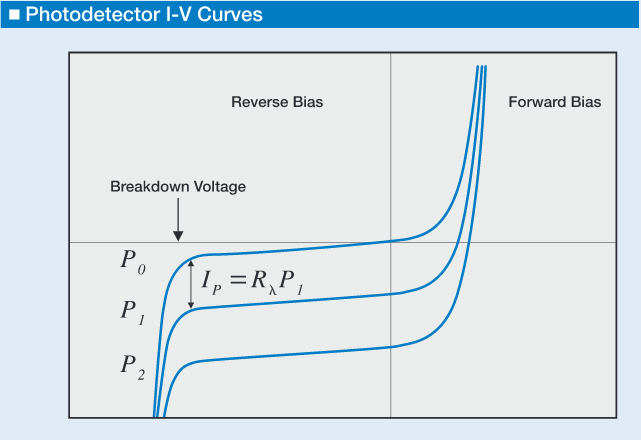
\includegraphics[width=3in]{diode-curve.png}
	\caption{Photoconductive Diode Curve~\cite{diode-curve}}
	\label{fig:diode-curve}
\end{figure}  

A transimpedance amplifier can be implemented to convert the current signal into a voltage signal making it quite easy to collect the resulting data using an analog-to-digital converter. However, since the analog-to-digital converter has a limit on the conversion rate, the frequency of the PZT must match this rate to achieve maximum resolution.


%-----------------------------------------------------------------
%   sFPI DESCRIPTION
%-----------------------------------------------------------------

\section{sFPI Description}
The scanning Fabry-Perot interferometer as discussed in Section~\ref{ss:background}, the optical design, the mechanical design, and the electrical design are the three key design parameters. The cavity design was chosen based on the typical construction for a Fabry-Perot interferometer. The mechanical design was ... The electrical design was based on the operation of the Spectra Physics Scanning Interferometer Driver which consisted of a signal generator with the ability to change the . 

% Optical Setup section

\section{Optical Design} \label{ss:optical_design}
The optical design component, as illustrated in the block diagram, is a Fabry-Perot interferometer. This resonant cavity consists of two spherical mirrors with a radius of curvature equal to 40 mm $\pm\;2$ mm. In order to have a stable cavity the following equation applies.

\begin{equation}
0 \leq \Big(1-\frac{L}{R_1}\Big)\Big(1-\frac{L}{R_2}\Big) \leq 1
\label{eq:unsolved_stability}
\end{equation}

Given that $R_1 = R_2 = 40\;\text{mm} \pm2\;\text{mm}$, the range of the length of the cavity ($L$), for a stable resonator, is:

\begin{equation}
0 \leq L \leq 40\;\text{mm} \pm 2\;\text{mm}
\label{eq:cavity_stability}
\end{equation}

The surface of the mirrors are coated with a dielectric material which has a reflectivity ranging from $99.4-99.8\%$ for 632.8 nm light. The finesse of this cavity, as explained in Section~\ref{ss:background}, is expected to be within the range of $522 - 1569$ for the respective reflectivity.  The resonant cavity for the device is represented in Figure~\ref{fig:auxlens}. 

% Mirror Setup
\begin{figure}[h!]
  \centering
	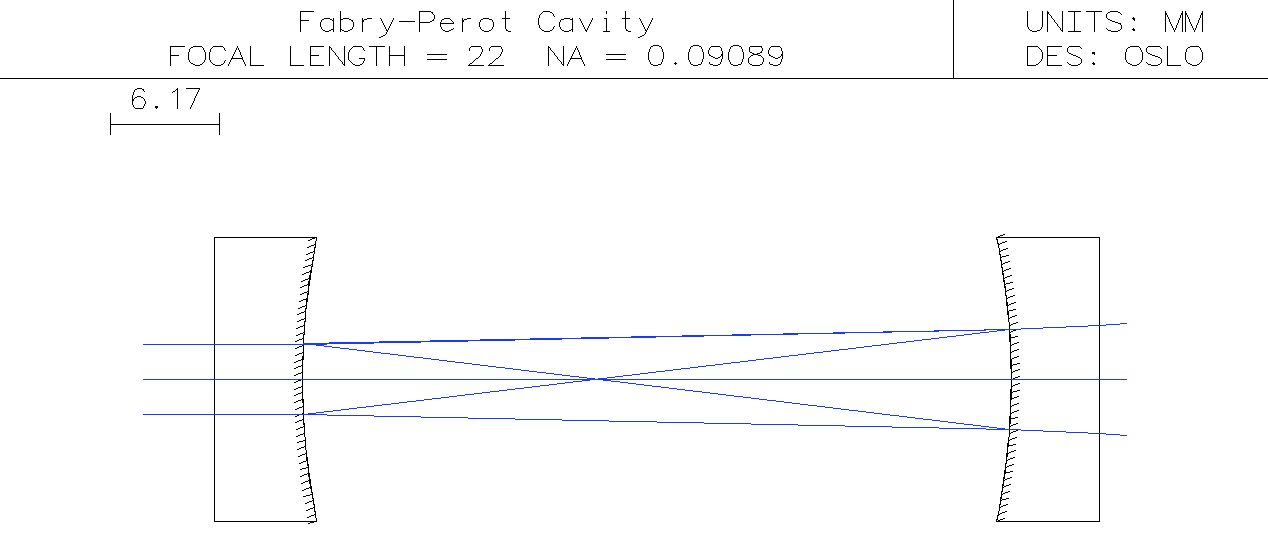
\includegraphics[width=3in]{./cavity/resonant_cavity.png}\\
	\caption[Resonant Cavity Setup]{The resonant cavity is comprised of two dielectrically coated spherical mirrors, which reflect 632.8 nm light with ~98\% reflectivity}
	\label{fig:mirror-setup}
\end{figure}

An 75 mm PCX lens is used to couple the system and account for any misalignment. By adding in the auxiliary lens the spot size of the output is decreased as well as the divergence angle of the gaussian beam leaving the cavity. Figures~\ref{fig:mirror-setup} and~\ref{fig:aux-mirror-setup} show the direct improvement of adding in an auxiliary lens to the system. This is done assuming a confocal resonant cavity with the focal point of the auxiliary lens matching the center of the resonant cavity.

\begin{figure*}[tb]
  \centering
	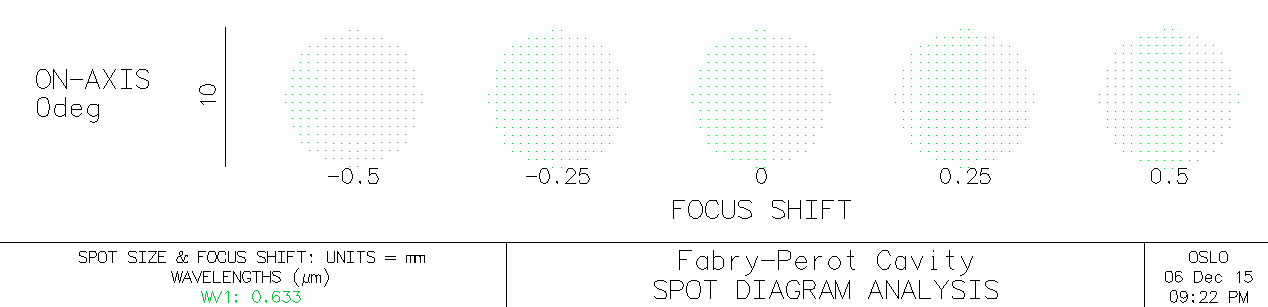
\includegraphics[width=6.5in]{./cavity/spot_size.png}\\
	\caption[Resonant Cavity Setup]{The spot size of the light exiting the resonant cavity after 1 pass}
	\label{fig:mirror-setup}
\end{figure*}

\begin{figure*}[tb]
  \centering
	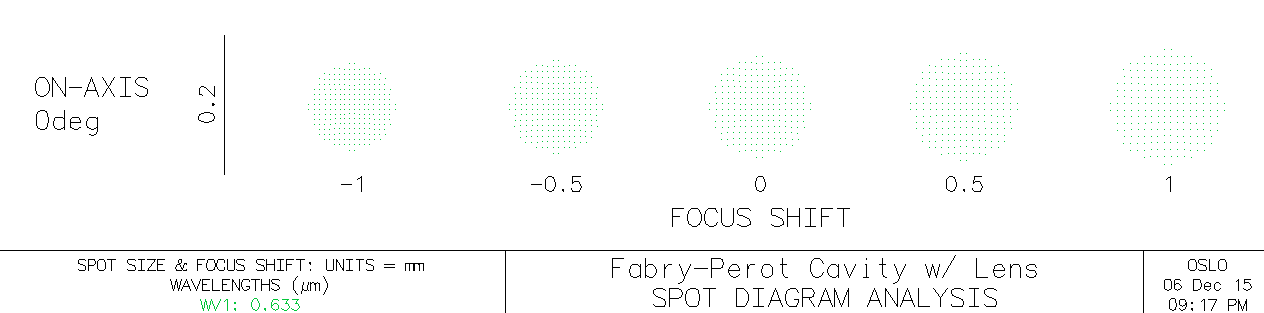
\includegraphics[width=6.5in]{./cavity/auxiliary_lens_spot_size.png}\\
	\caption[Resonant Cavity Setup]{The spot size of the light exiting the resonant cavity after 1 pass with an auxiliary lens of 75 mm focal length}
	\label{fig:aux-mirror-setup}
\end{figure*}

% Beam Diameters
\begin{figure}[h!]
  \centering
	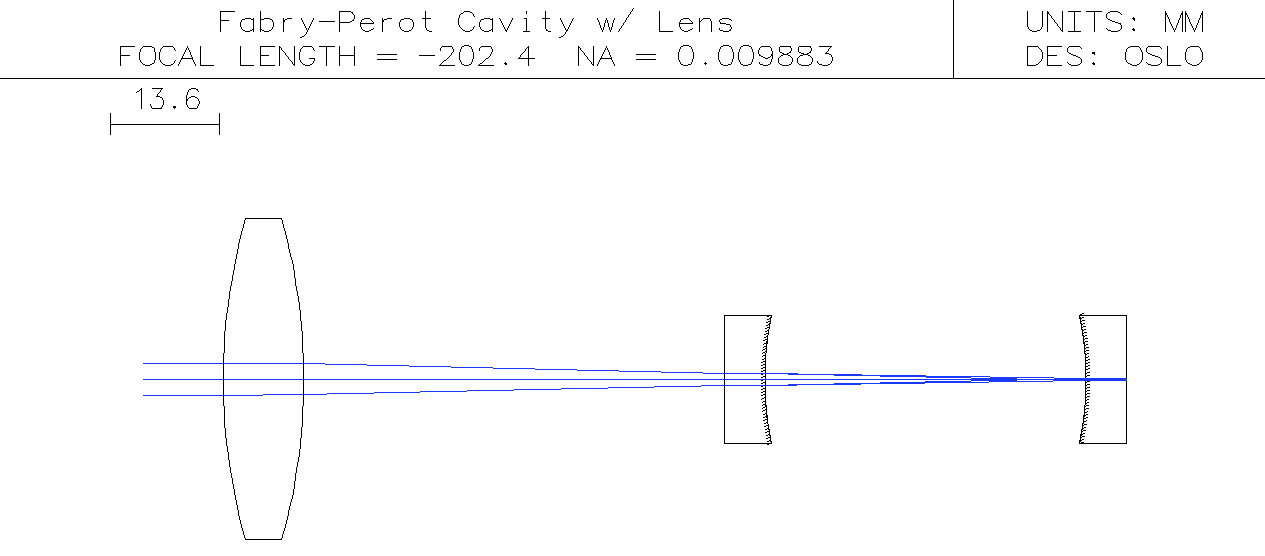
\includegraphics[width=3in]{./cavity/auxiliary_lens_resonant.png}\\
	\caption[Auxiliary Lens Setup]{The auxiliary lens couples the incoming beam to the resonant cavity by increasing the photon-lifetime of the cavity}
	\label{fig:beam-diameter}
\end{figure}

% Image of that

\section{Mechanical Design} \label{ss:mechanical_design}

The first surface mirror is mounted in a milled disk which is counter sunk, to keep the mirror from falling out (see Figure~\ref{fig:fsm}). This is held in place by a set screw. 

\begin{figure}[h!]
  \centering
	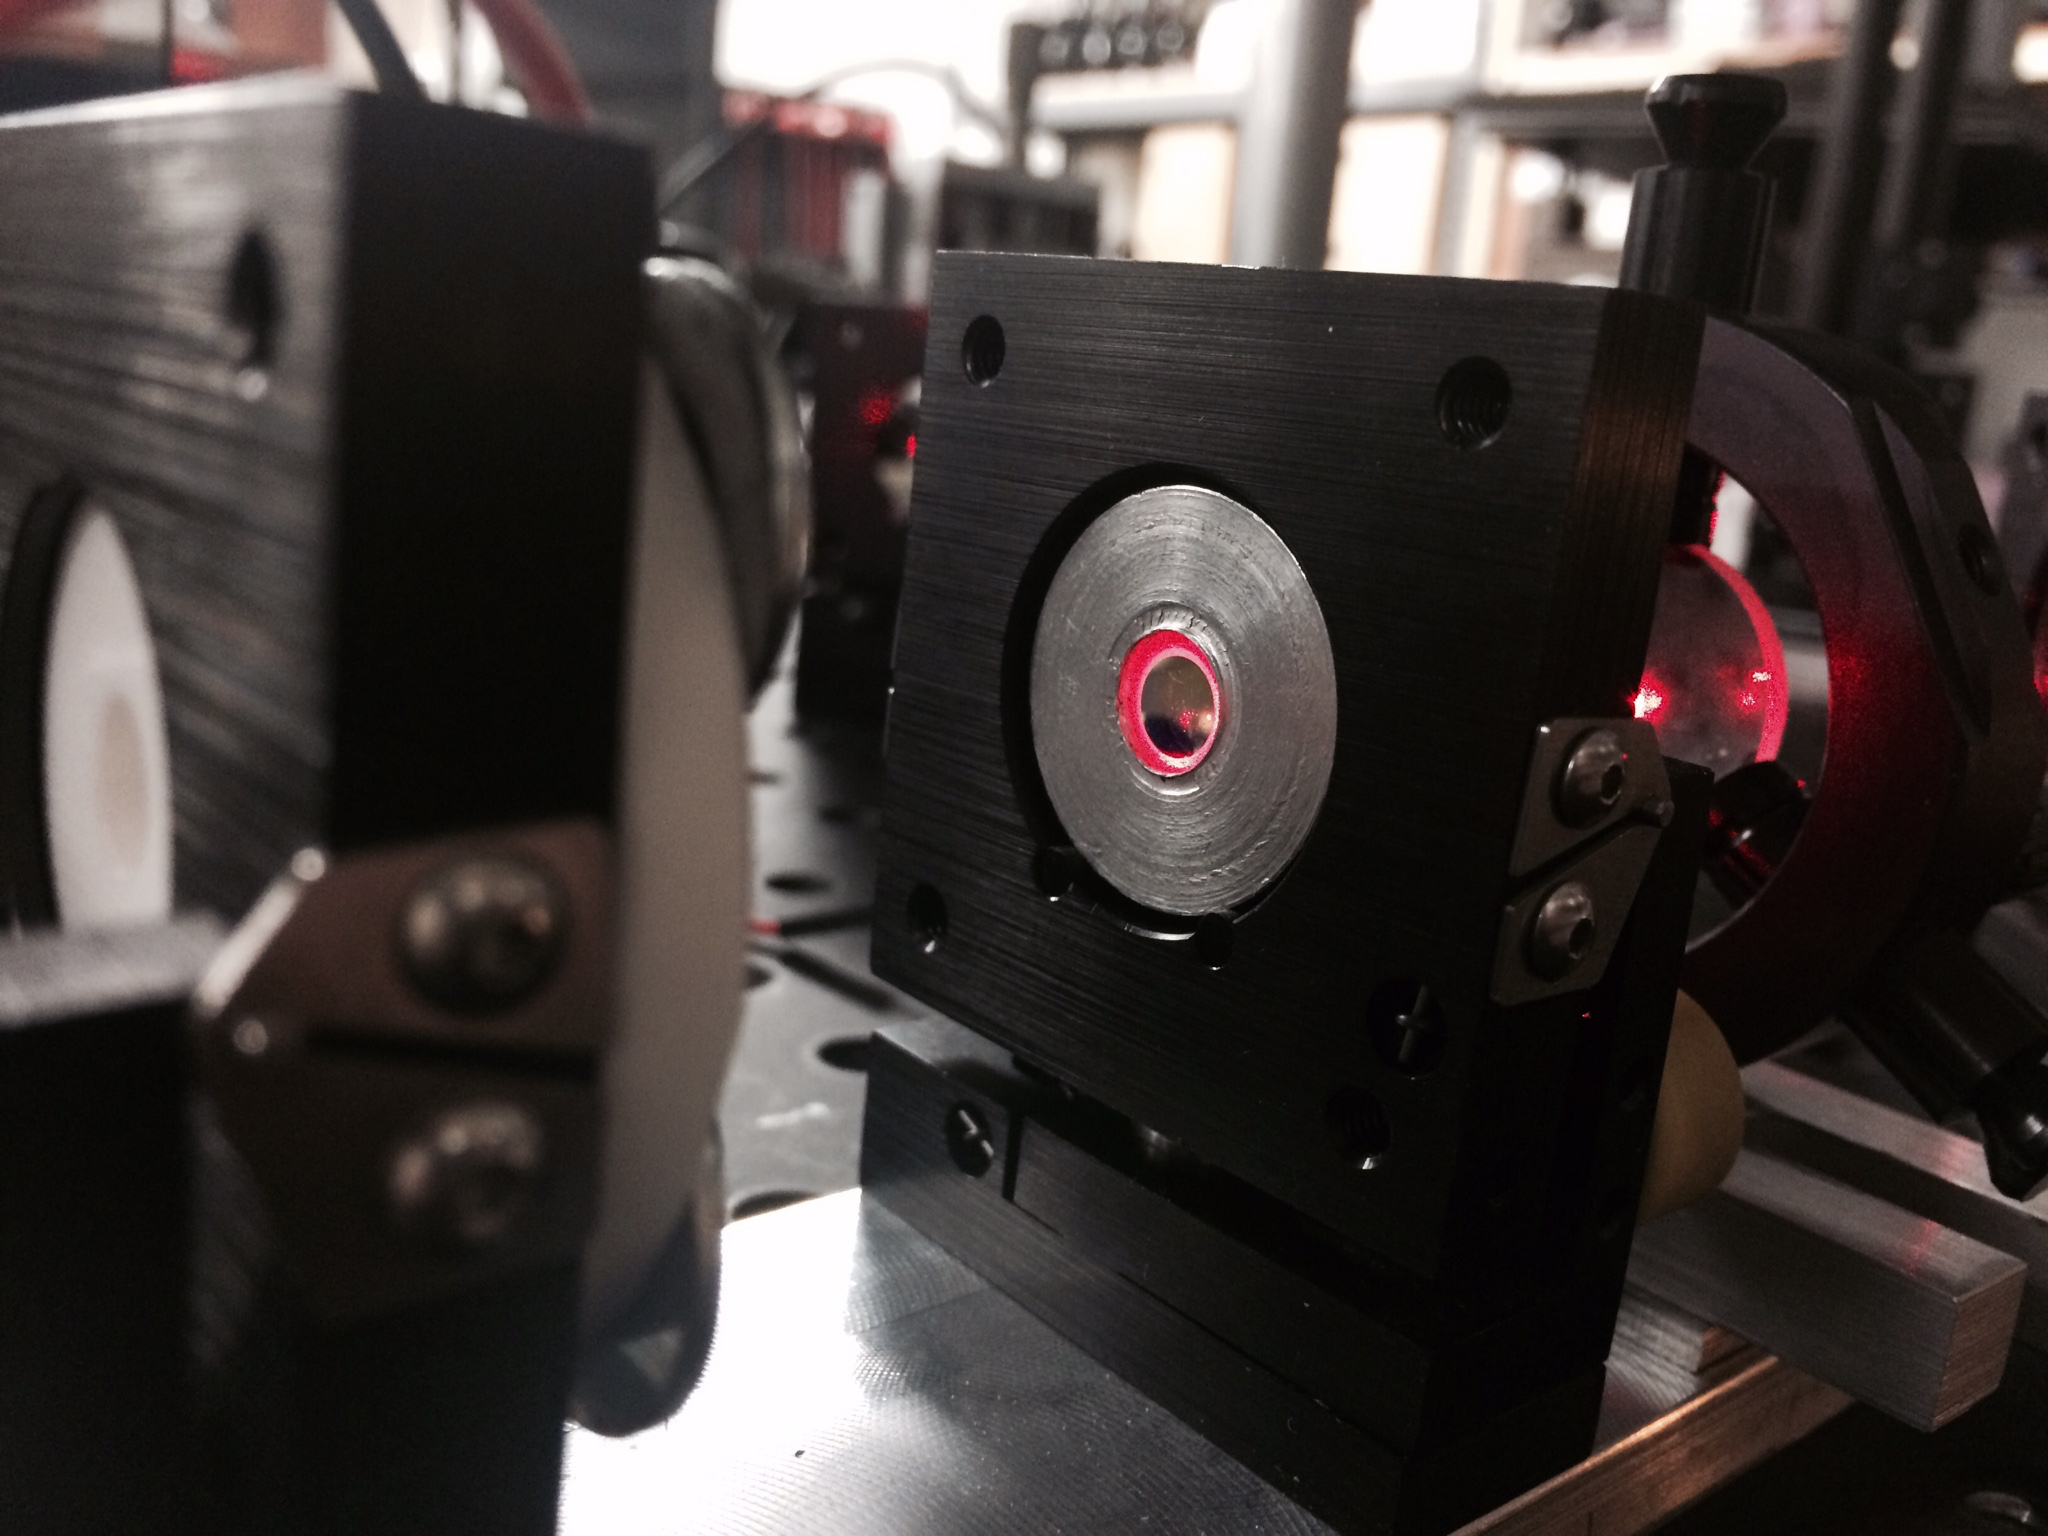
\includegraphics[width=3in]{first-lens-holder.png}
	\caption{Milled Disk for first surface mirror}
	\label{fig:fsm}
\end{figure}

The second surface mirror is attached to the piezo-electric device, which is described in more detail in the next subsection. This is done by the clear adhesive Gorilla Glue. The piezo-mirror combination is mounted to a plastic appendage (Figure~\ref{fig:holder}). This plastic appendage is designed to keep the limiting aperture within the cavity, when properly aligned. It is designed such that 4 washers hold the Piezo-Mirror combination in place, without grounding the plates, and so that it fits inside the adjust mounts (see Figure~\ref{fig:plastic-mount-piezo-mirror}).  

\begin{figure}[h!]
   \centering
   	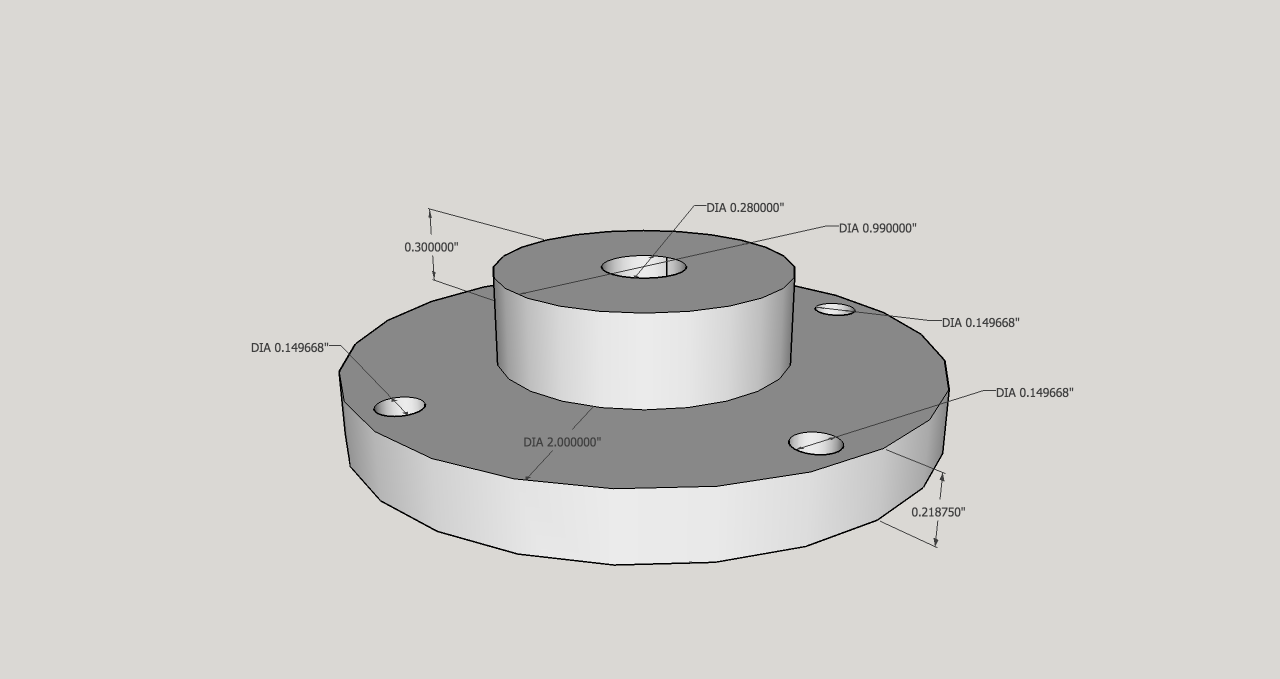
\includegraphics[width=3in]{./mechanical/PZT_holder_3d_rep.png}
	\caption{Piezo-Mirror Holder}
	\label{fig:plastic-mount-piezo-mirror}
\end{figure}

\begin{figure}[h!]
  \centering
	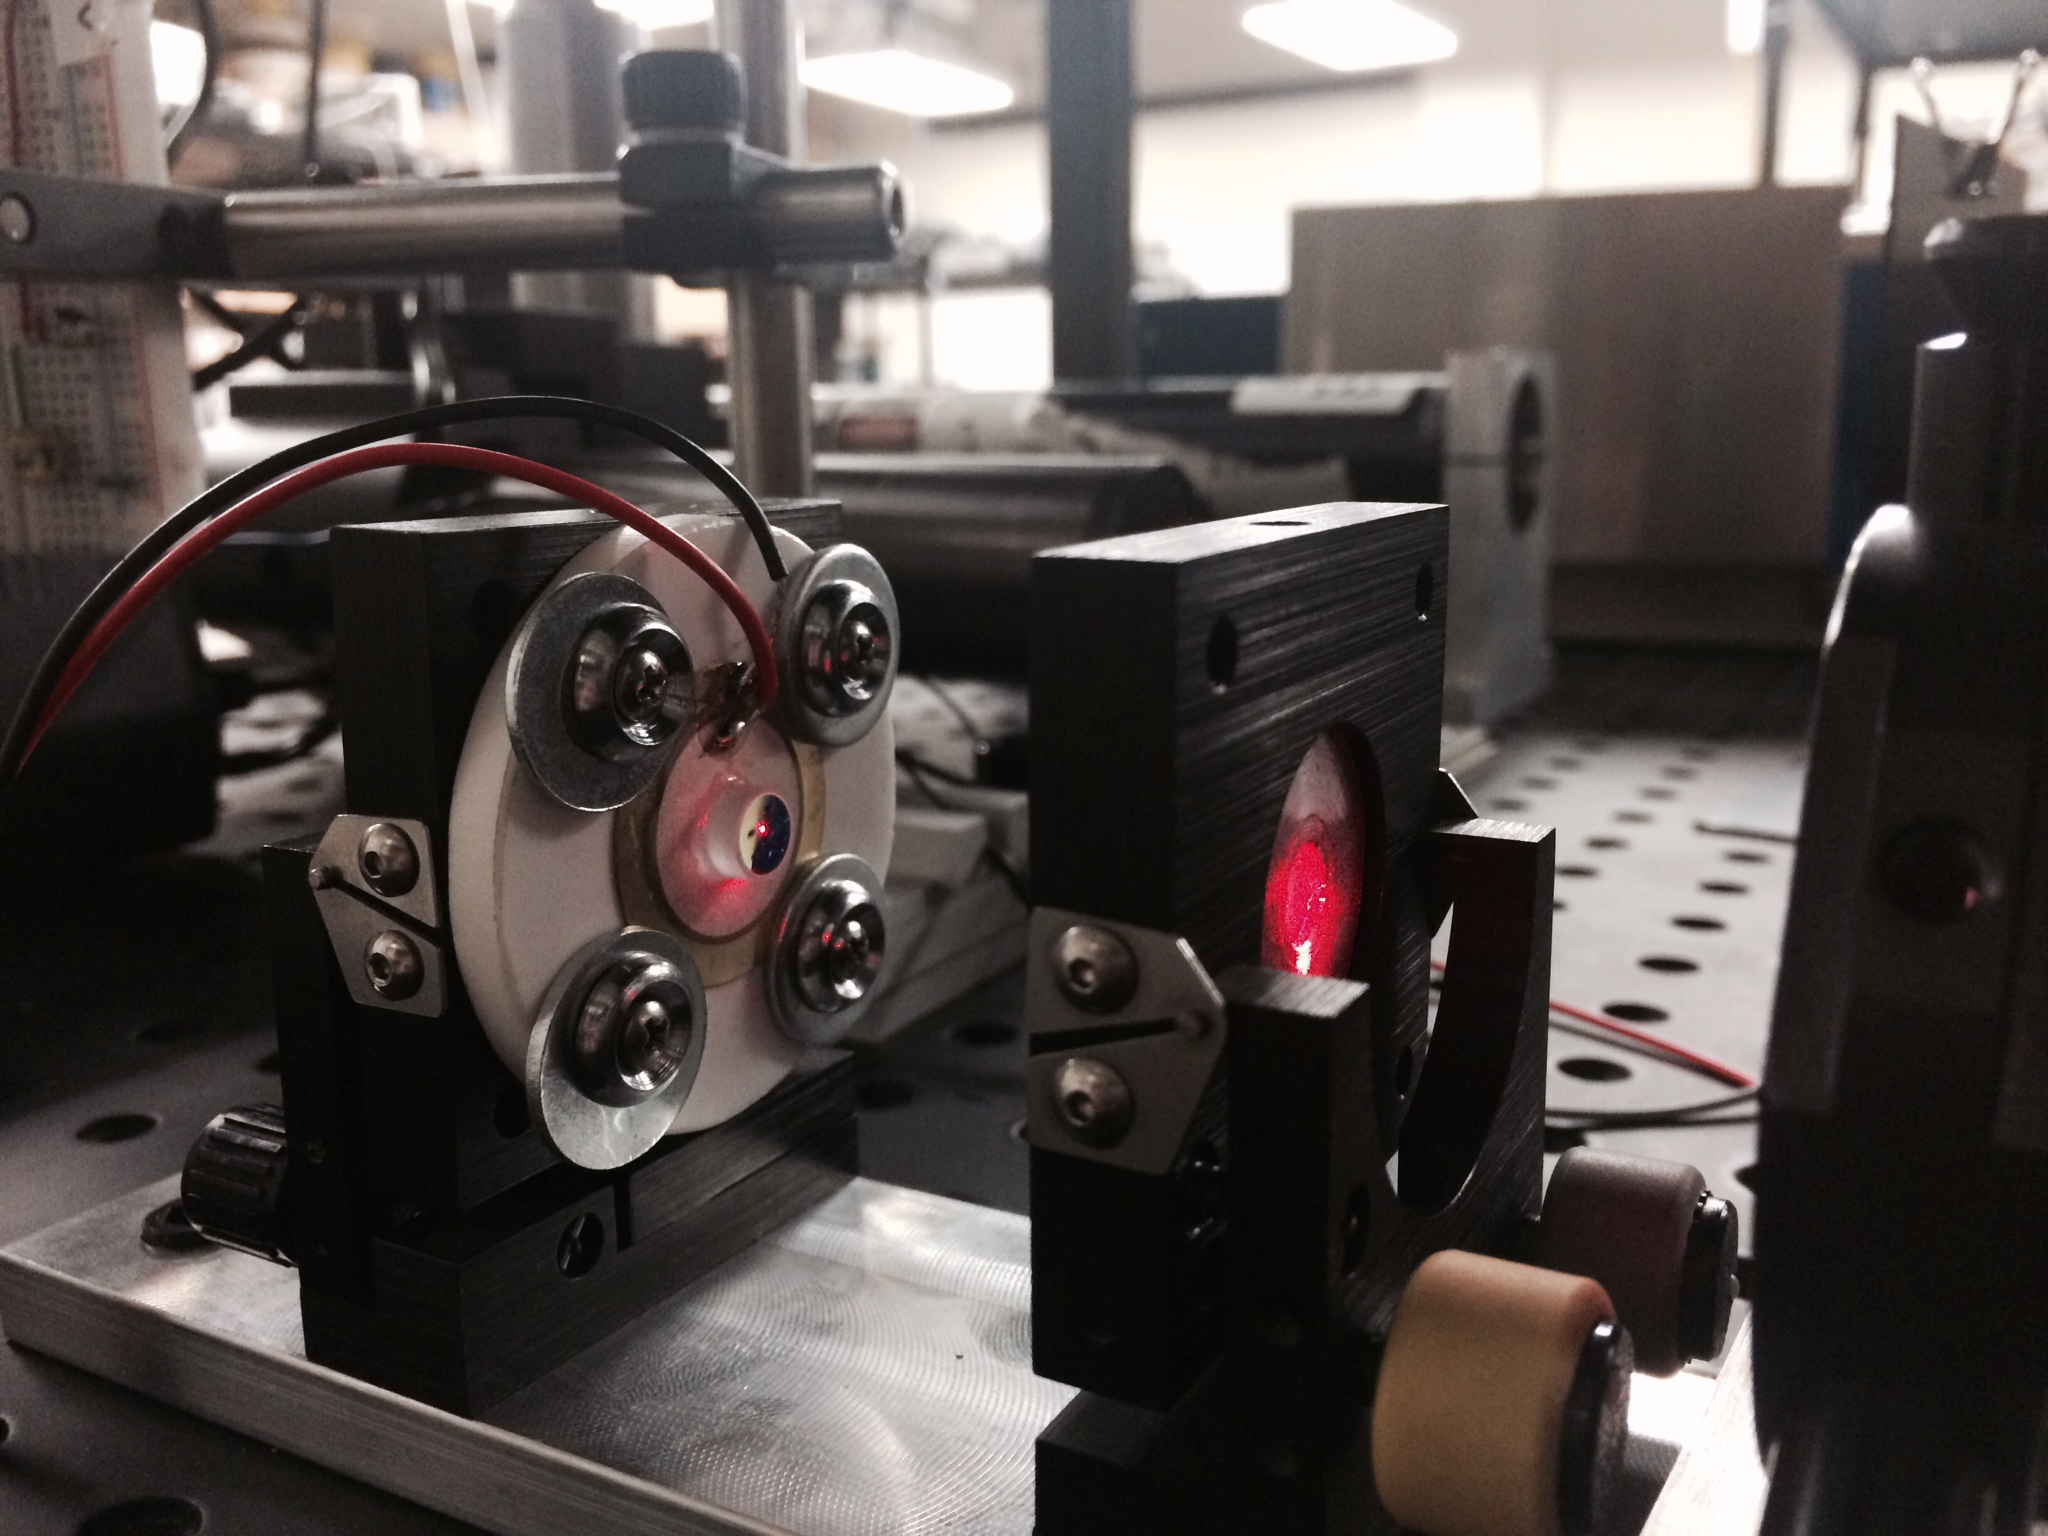
\includegraphics[width=3in]{second-surface-holder.png}
	\caption[Second-Surface Piezo-Mirror Holder]{Piezo-Mirror Holder Dimensions}
	\label{fig:holder}
\end{figure}

The entire cavity is held in place by dual-axis adjustable mounts for aligning purposes (See Figure~\ref{fig:full-cavity}). These are attached to an aluminum base with adjustable distances between the mirrors (Figure~\ref{fig:base}).

\begin{figure}[h!]
  \centering
	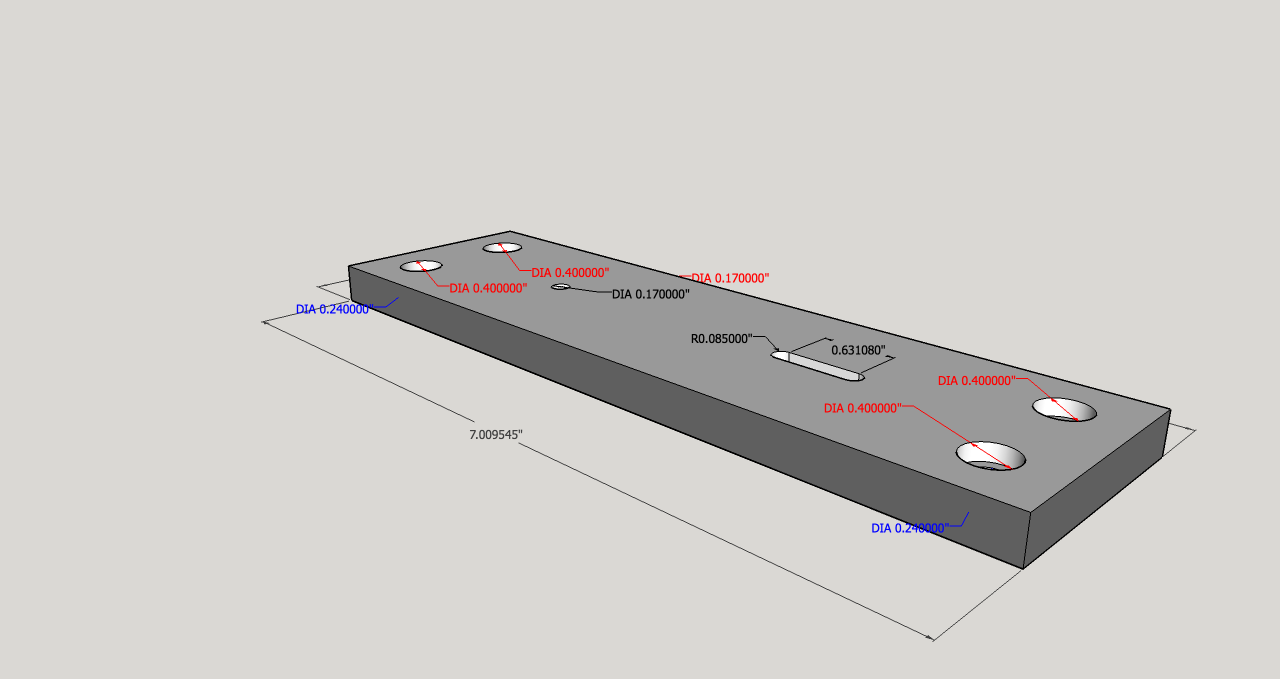
\includegraphics[width=3in]{./mechanical/sfpilensholder_3d_rep.png}
	\caption[Cavity Mounts]{Aluminum base for the sFPI cavity system. Full layout drawings with measurements can be found in on page~\pageref{ss:sfpilensholder}}
	\label{fig:full-cavity}
\end{figure}

\begin{figure}[h!]
  \centering
	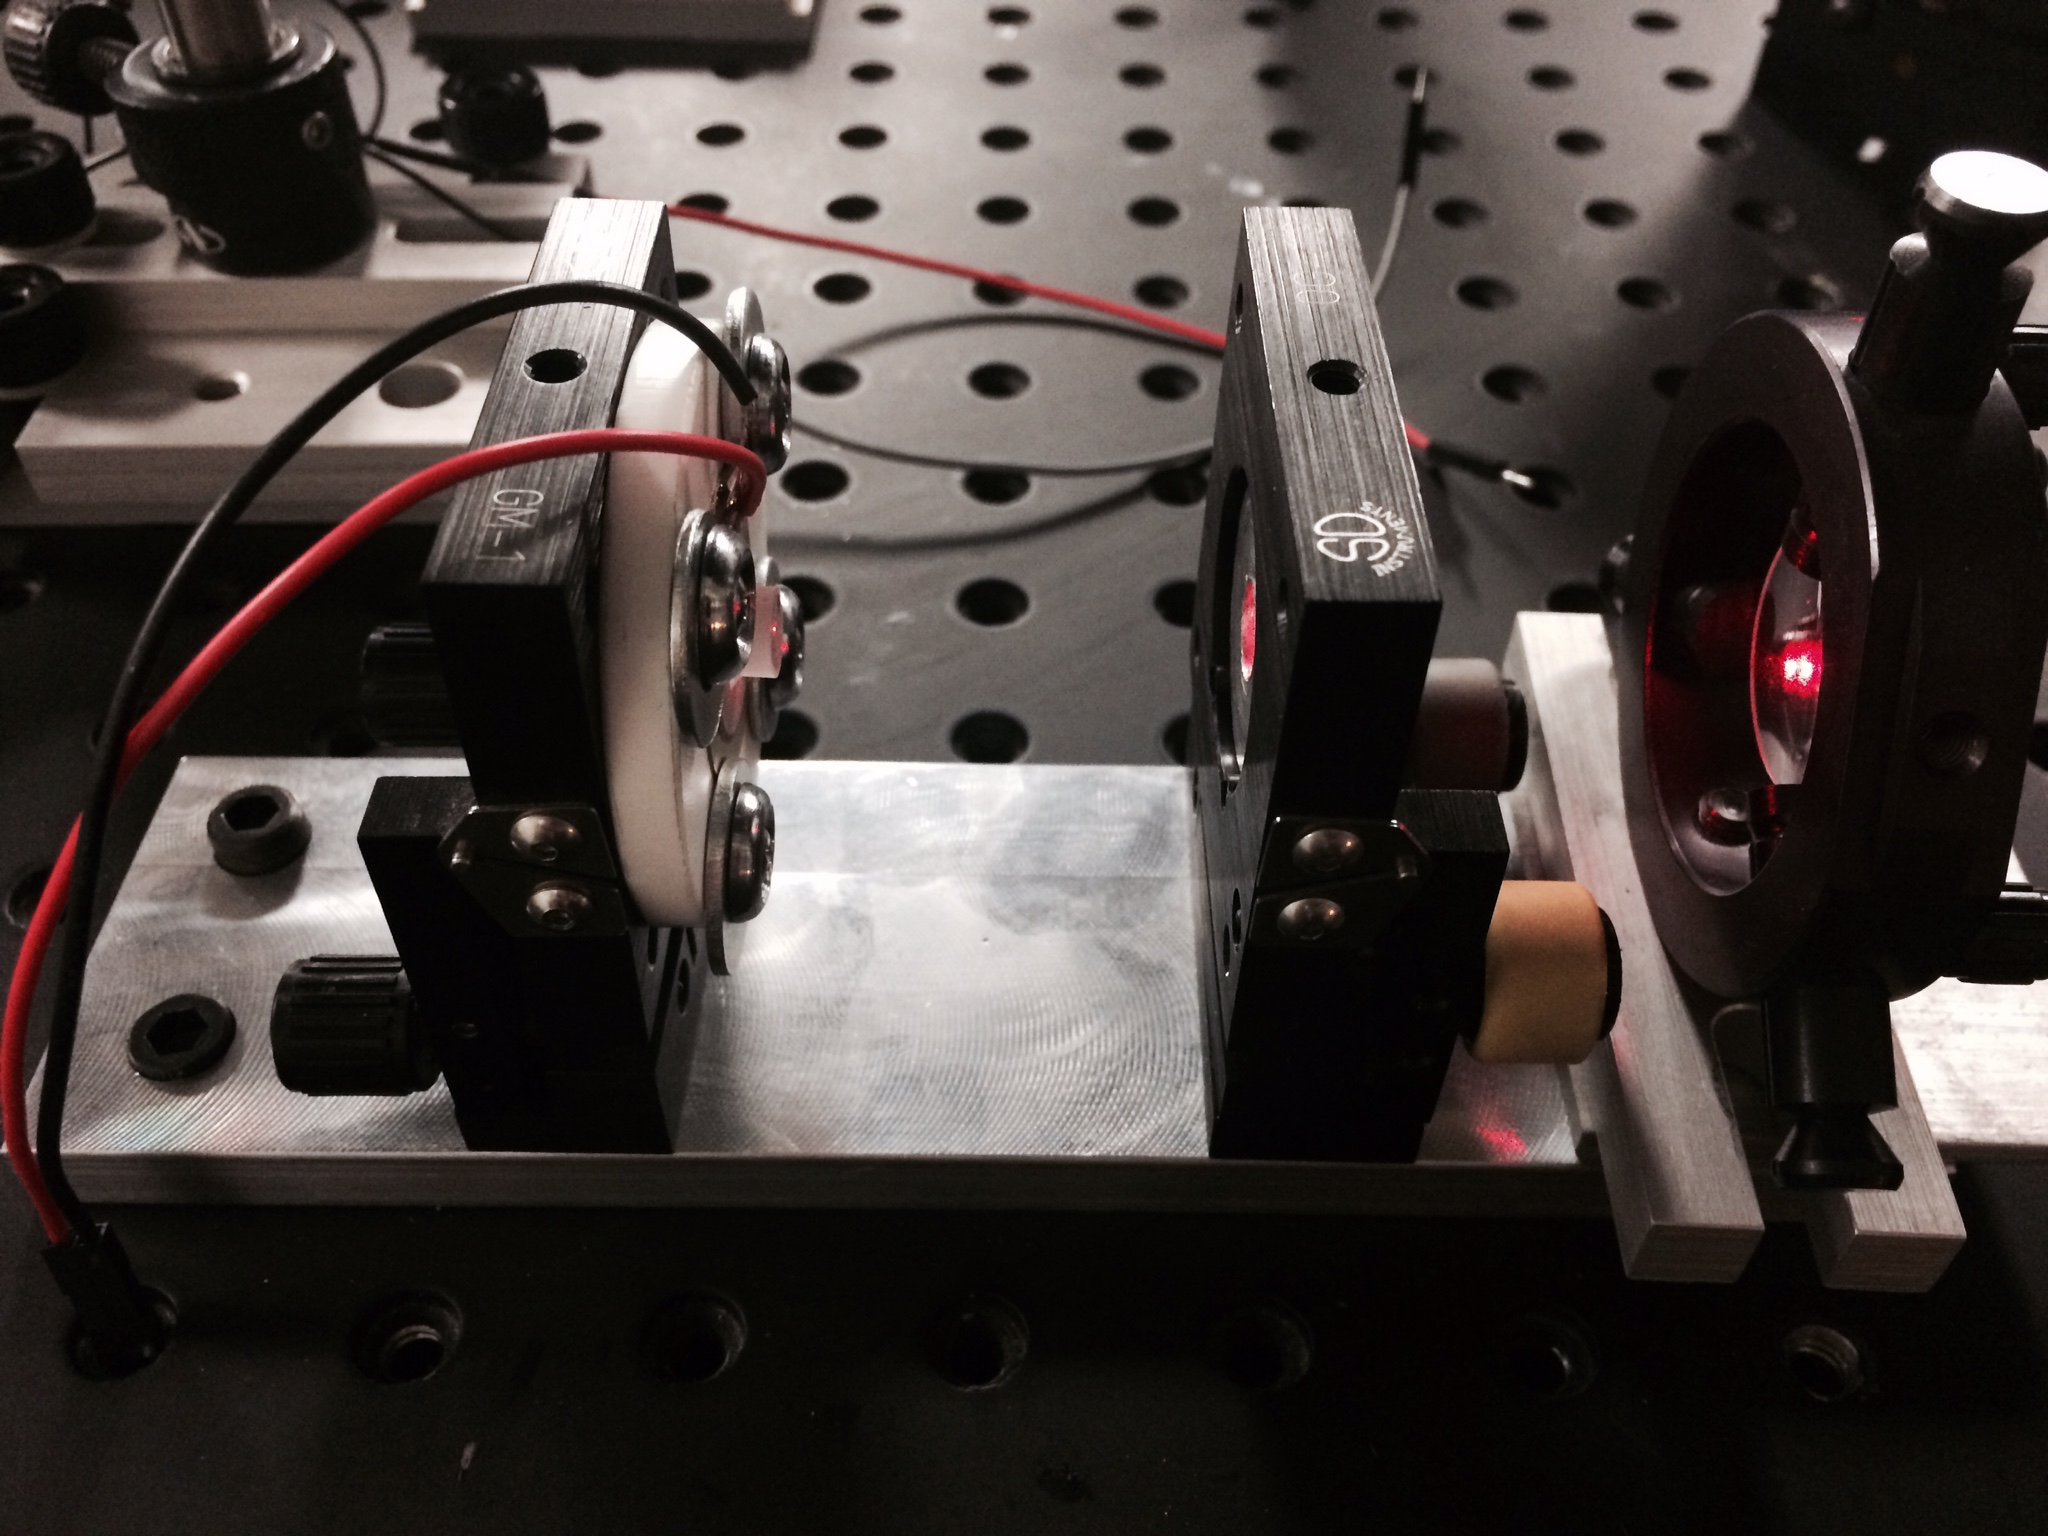
\includegraphics[width=3in]{full-cavity.png}
	\caption[Cavity Mounts]{Adjustable mounts for entire cavity setup}
	\label{fig:full-cavity}
\end{figure}

The photodiode is mounted on the back of the adjustable mounts (Figure~\ref{fig:mounts-holder}) by the specially made holder (Figure~\ref{fig:diode_holder}). A set screw is taped post-3D-print in order to secure the photodiode. This is done with a 4-40 drill and tap for a 4-40 set screw. 

\begin{figure}[h!]
  \centering
	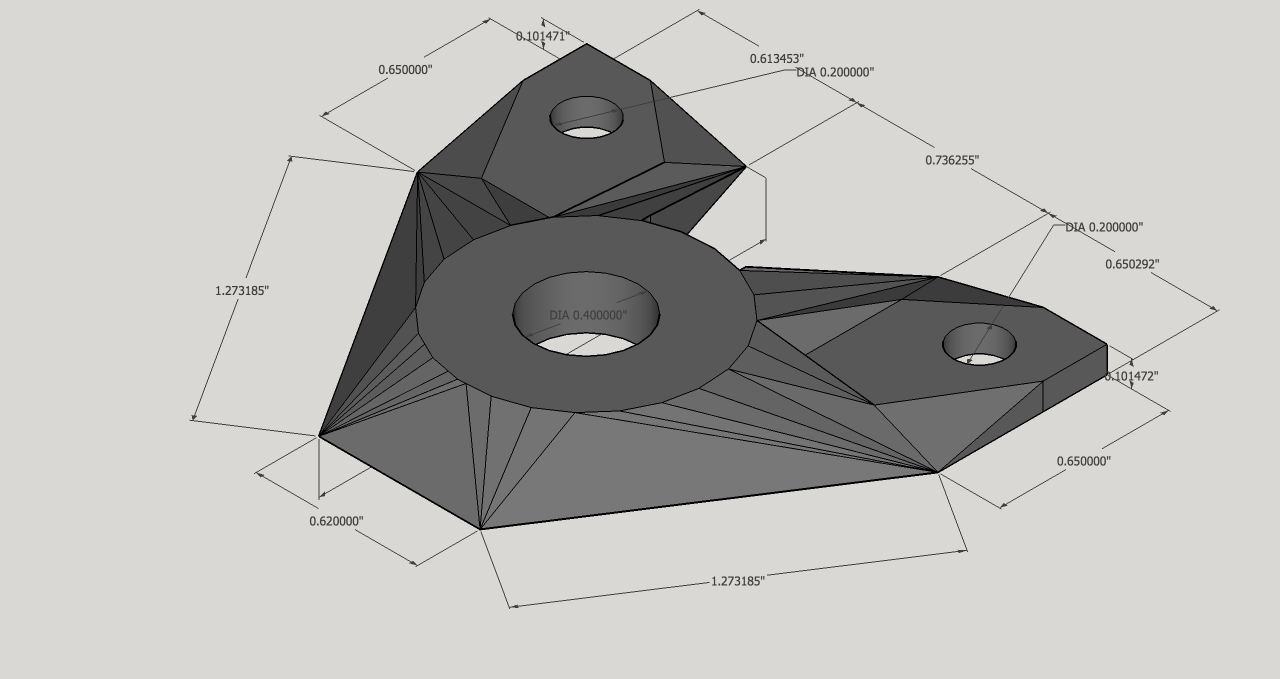
\includegraphics[width=3in]{./mechanical/diode_holder_3d_rep.png}
	\caption[Cavity Mounts]{The mounting device for the photodiode with all measurements and outlays specified on page~\pageref{ss:diode_holder}}
	\label{fig:diode_holder}
\end{figure}

\begin{figure*}[tb]
  \centering
	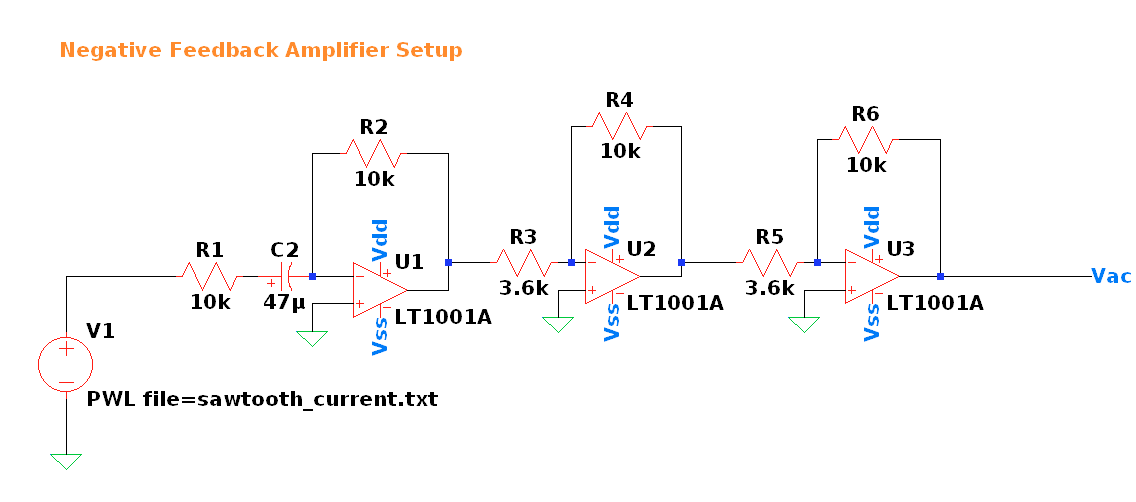
\includegraphics[width=6in]{/ltspice/amplifier-circuit-design-ltspice.png}
	\caption[Cavity Mounts]{The three-stage negative feedback amplifier configuration provides a range of 0.2 V/V up to 7.716 V/V of amplification to the input signal by changing resistors R3 and R5 from $3.6\;k\Omega$ to $10\;k\Omega$. $V_{DD}$ and $V_{SS}$ are the respective positive and negative voltage rails +17V and -17V. For more clarification the full LTSpice model is Figure~\ref{ltspice:driver} in Section~\ref{ss:ltpsice-models}}
	\label{fig:amplifier-configuration}
\end{figure*}

\section{Interferometer Driver Design}

\subsection{Function Generator}
The micro-controller for the driver setup is constructed using an Arduino UNO (see Data Sheet on page~\pageref{datasheet:arduino_uno}). The Arduino UNO has firmware in which it communicates with a MCP4725 (see Data Sheet on page~\pageref{datasheet:mcp4725}) 12-bit Digital-to-Analog Converter (DAC) via the I2C communication protocol (see Figure~\ref{fig:function-generator}).The DAC attenuates the +5V 10\% voltage supply from the Arduino UNO with $2^12$ individual output values. A peak-to-peak sawtooth voltage signal is the result, with a bit resolution of 1.2 mV/bit at a frequency of 2.5 Hz (see Figure~\ref{fig:five-volts-15-hz-wave}). The MCP4725 signal-generator acts as a near-perfect voltage source with a series impedance of $1\Omega$ when in normal operations. This will not affect input resistances for the analog design.  

\begin{figure}[h!]
  \centering
	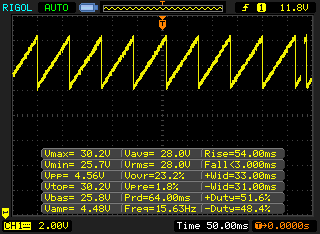
\includegraphics[width=3in]{./data/dac-output-waveform.png}
	\caption[Cavity Mounts]{The output of the MCP4725 DAC from the I2C communication with the Arduino which has 4096 individual steps from $0-5 \pm 10\% V$}
	\label{fig:five-volts-15-hz-wave}
\end{figure}

\subsection{Analog-Amplifier Circuit}

The sawtooth waveform is sourced to a three-stage negative feedback amplifier configuration (Figure~\ref{fig:amplifier-configuration}). The amplification ($A_v$) is adjustable from $0.2 V/V$ up to $7.716 V/V$. This is done through three stages: the dispersion stage and the two magnitude stages. The dispersion stage allows for small adjustments, 0.2x to 1x of the original signal based on $R_{in_{min}} = 10k\Omega$ and $R_{in_{max}} = 50k\Omega$. The magnitude stage allows for 1x to 3x of the original signal based on  $R_{in_{min}} = 3.6k\Omega$ and $R_{in_{max}} = 10k\Omega$. 

Resistors R1, R2, and R3 are representation of an array of resistors. Figure~\ref{fig:r1-array} details the configuration of R1, which is the adjustable input resistance of the dispersion stage of the amplifier.

\begin{figure}[h!]
  \centering
	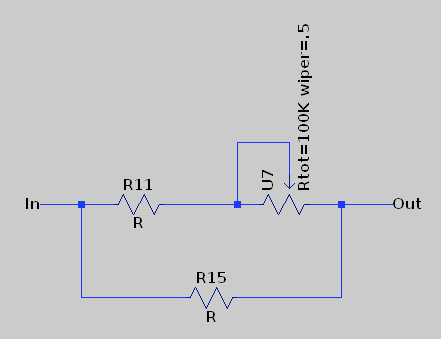
\includegraphics[width=3in]{./ltspice/adjustable-resistor-array.png}
	\caption[Cavity Mounts]{This is the array of resistors which}
	\label{fig:r1-array}
\end{figure}

has  which are complimented by a 100k potentiometers having an effective range of $0-100k\Omega$This increases the AC range from 5 volts to 34 volts. Adjustment of this gain is done by a series of potentiometers governed by Eq.~\ref{eq:pot}.

\begin{equation}
A_v = (R_f)^3\Big(\frac{1}{R_1}\Big)\Big(\frac{1}{R_2}\Big)\Big(\frac{1}{R_3}\Big)
\label{eq:pot}
\end{equation}

A LTSpice Netlist program was developed (see code on page~\pageref{code:ltspice-driver}). This provided the expected output of the signal given a specified input signal. This input signal is generated by a python-shell script which generates a PWL file for LTSpice based on a series of user inputs (see code on page~\pageref{code:pwl-ltspice-python}).

This is sourced to a buffer which uses a single NTE941M (see Datasheet on page~\pageref{datasheet:nte941m}) operation amplifier. This gives the AC signal an infinite output impedance, preventing impedance mismatching. Figure~\ref{fig:buffer} denotes the circuit construction.

\begin{figure}[h!]
  \centering
	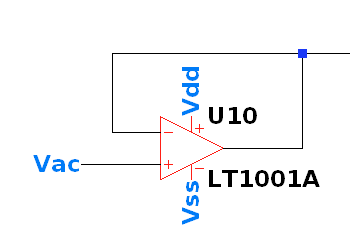
\includegraphics[width=3in]{./ltspice/unity-buffer-ltspice.png}
	\caption[Cavity Mounts]{The voltage follower (unity buffer amplifier) configuration for an OpAmp for circuit isolation and prevention of impedance mismatching.}
	\label{fig:buffer}
\end{figure}  

To change the offset biasing of the sawtooth voltage signal an NTE957 (see Datasheet on page~\pageref{datasheet:nte957}) adjustable DC voltage regulator is added using a summation circuit to the AC signal with the following configuration (Figure~\ref{fig:dc-adj-voltage}).

\subsection{Power Distribution}

A VELLEMAN PSINO2512N 12-VOLT 25-WATT DC SWITCHING POWER SUPPLY (see Datasheet on page~\pageref{datasheet:psino2512n}) was complimented with a DROK Micro Electric DC/DC Boost Converter LM2577 Step-up Voltage Transformer (see Datasheet on page~\pageref{datasheet:drok} for specifications of the DROK component and on page~\pageref{datasheet:lm2577} for the LM2577 data sheet) to provide the power to the system. A NTE1234 5 VDC $\pm 1\%$ fixed voltage regulator (see Datasheet on page~\pageref{datasheet:nte941m}) and an MAX737 inverting buck-boost converter (see Datasheet on page~\pageref{datasheet:max737}). 

The 12VDC PSIN02512N voltage supply is sourced to LM2577, boosting the voltage to 17 VDC. The 17 VDC is sourced to the NTE1234 5-VDC producing +5 volts suppling power to the boot-loaded Arduino and the MCP4725 DAC. 

Since the design calls for a signal with a max peak-to-peak voltage of approximately 34V, the rails must have a range +17 VDC to -17 VDC. Since the constraint that $V_s - V_out \leq 22 V_DC$ holds for the buck converter, if the 5VDC rail is used, $V_{out_{max}} = -17 V$~\cite{datasheet_max635}. This is achieved by using values for $R_3 = 92\;k\Omega$ and $R_4 = 1.2\;M\Omega$ (Figure~\ref{fig:power-distribution}). 

\begin{figure*}[tb]
  \centering
	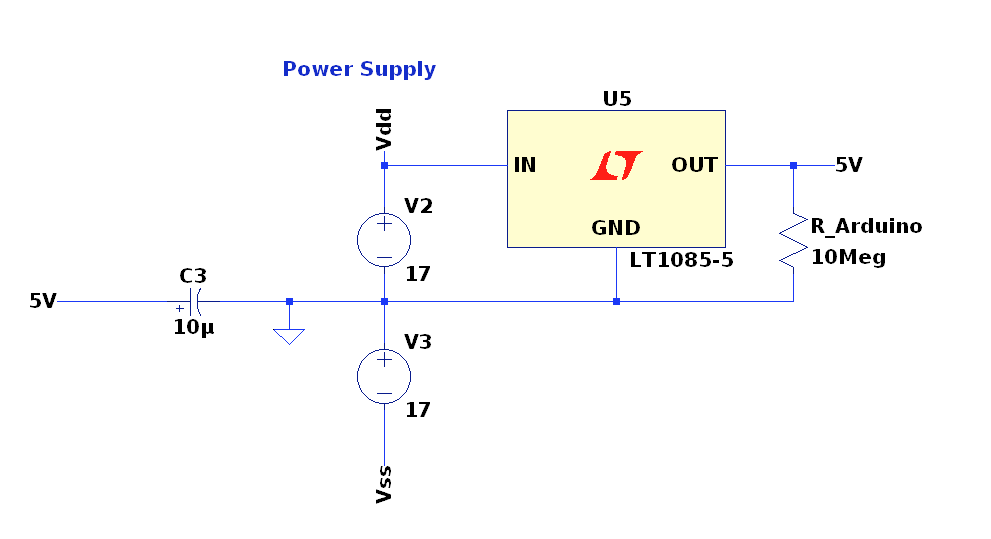
\includegraphics[width=6in]{/ltspice/power-supply-circuit-desgin-ltspice.png}
	\caption[Cavity Mounts]{The three-stage negative feedback amplifier configuration provides a range of 0.2 V/V up to 7.716 V/V of amplification to the input signal by changing resistors R3 and R5 from $3.6\;k\Omega$ to $10\;k\Omega$. $V_{DD}$ and $V_{SS}$ are the respective positive and negative voltage rails +17V and -17V. For more clarification the full LTSpice model is Figure~\ref{ltspice:driver} in Section~\ref{ss:ltpsice-models}}
	\label{fig:amplifier-configuration}
\end{figure*}

The current design of the board, which will be discussed later in this section, was simulated in LTspice for power consumption calculations. The negative power supply was sinking 22.69 mA of current. In order to calculated the range of inductance necessary for operations Eqs~\ref{eq:ipk} and~\ref{eq:l} were used. 

\begin{equation}
I_{pk} = \frac{4(V_{out} + V_{DIODE})}{V_{in} - V_{sw}}*I_{out}
\label{eq:ipk}
\end{equation}

\begin{equation}
L = \frac{V_{in} - V_{sw}}{I_{pk}}*t_{on}
\label{eq:l}
\end{equation}

$I_{pk}$ was found to be 426.8 mA. This is significantly less than the max current rating of 525 mA; therefore a current source is not necessary to complete this setup. Given that the switching time ($t_{on}$) for the converter is roughly $10\;\mu s$ the range of inductors was found to be $73.8\; \mu H \leq L \leq 105\; \mu H$.  

\section{Analog Data Conversion Processor}\label{processor}
The photodiode is mounted to an adjustable plate at the rear of the sFPI for calibration, for maximum transmission of the spectral content. The photodiodes resulting current is reverse biased by an Arduino UNO (\#2), which is supplying the 5V. Based on the IV curve of the photodiode, the voltage stays within the photoconductive range while remaining far enough away from the breakdown voltage. 
\\\\
A recent Ph.D. thesis details the quantum efficiency of doped GaAs being between 30\% and 22\%~\cite{responsivity}. This means at 632.8 nm a good approximation for the responsivity is 154 mA/W. The incident power on the detector can be approximated based on the losses in the cavity. Section~\ref{ss:optical_design} explained that the reflectivity of the mirrors was between $99.4\% - 99.8\%$. From this the transmitted power of the beam can be calculated for one pass through the cavity:

\begin{equation}
P_{out} = T_1T_2*P_{in}
\end{equation}

Given the ranges for reflectivity given above, that $T = 1-R$, and $P_{in} = 3 mW$, the output power of the cavity was found to be $P_{max} = 0.108 \mu W$ and $P_{min} = 120 nW$. With an optical output of approximately $1\;\mu W$ results in a current of roughly $0.154\;\mu A$.  
\\\\
A transimpedance negative-feedback amplifier with a voltage booster (TAV) converts the AC-current signal to a AC-voltage signal. The voltage gain of this amplifier setup is adjustable for tuning the sFPI, when the signal-to-noise ratio is small, to increase the intensity of the output of the cavity (Figure~\ref{schm:photodiode}). This corresponding output is sampled by an analog-to-digital converter (ADC). Since the Arduino, the micro-controller used for storing the data, uses a pre-scaler of 128, the ADC clock speed is set at 125 kHz. Given that it takes 13 ADC clocks for a conversion the ADC can sample data at a rate of 9615 Hz. Since our we have 4096 individual steps, to match the rate of the ADC a frequency of 2.35 Hz in used for the driver.    

\section{Digitally Analyzed Output}\label{digital-output}
The content captured by the ADC (Figure~\ref{schm:photodiode}) is transmitted to a computer to process, display (by a graphical representation), and stores the data by user command.  

\subsection{ADC-Computer Interface}
The voltage signal from the TAV is sampled by the Arduino Uno, as discussed in Section~\ref{processor}. This is converted to a 512 byte array. The array is then encoded to send to the computer upon request (see code in Section~\ref{serial-data}).

\subsection{Data Analysis}

This data will be combined in conjunction with the 5V sawtooth signal to plot the photodiode signal as a function of the geometrical change of the resonant cavity, which is proportional to the wavelength of the light. This will be done via a GUI model with a language that possesses the capability for universal interfacing. Python will be the base model for programming; however, other languages will be tested for user interface and compared based on speed, cross-platform configuration, and simplicity.

\section{Discussion}
In order to determine the quality of the sFPI data was collected, analyzed and compared with that from the SP-470-04 Interferometer for comparison. (Show data and the conclusions drawn from it).

\section{Conclusion}
Throughout this document we described a low-cost version of a sFPI. (Talk more, once more data is collected).

\bibliography{OIT_Thesis}

\begin{appendices}
\onecolumn

\section{Mechanical Assembly Drawings}
\subsection{PZT-Mirror Holder}

\begin{figure}[h!]
  \centering
	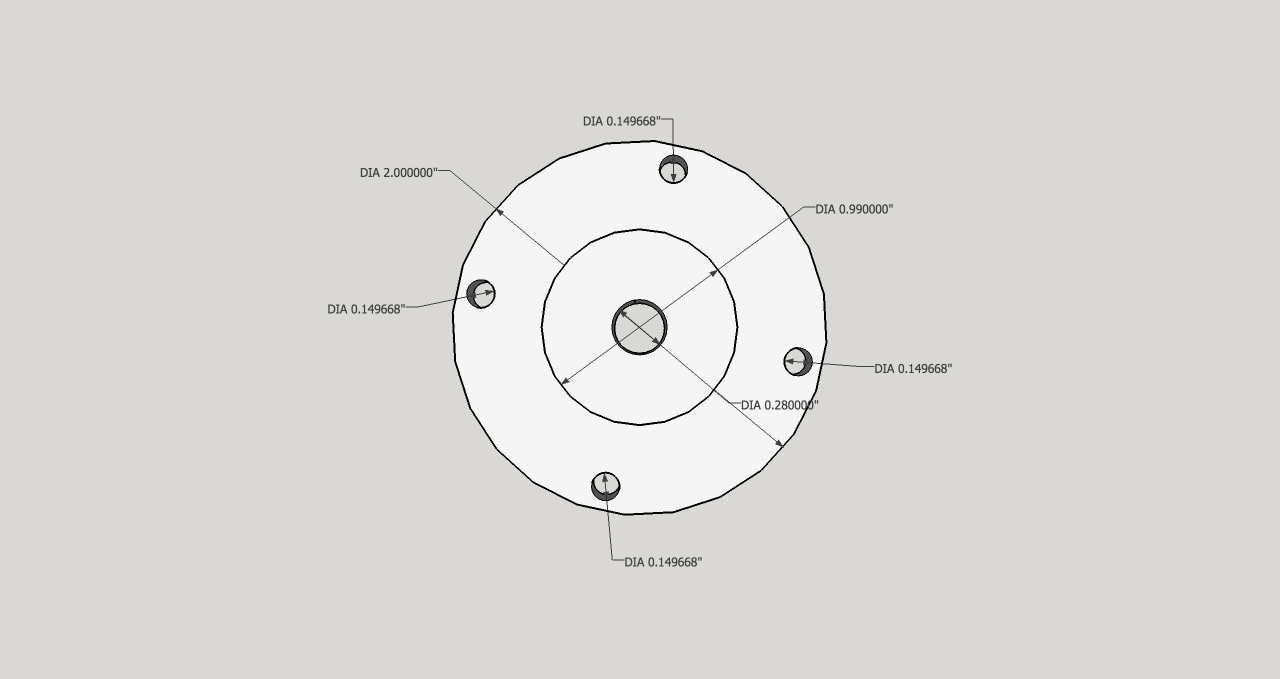
\includegraphics[width=\textwidth]{./mechanical/PZT_holder_top.png}
	\caption[Cavity Mounts]{The top down view and measurements of the PZT-Mirror holder}
	\label{fig:PZT-holder-top}
\end{figure}  

\begin{figure}[h!]
  \centering
	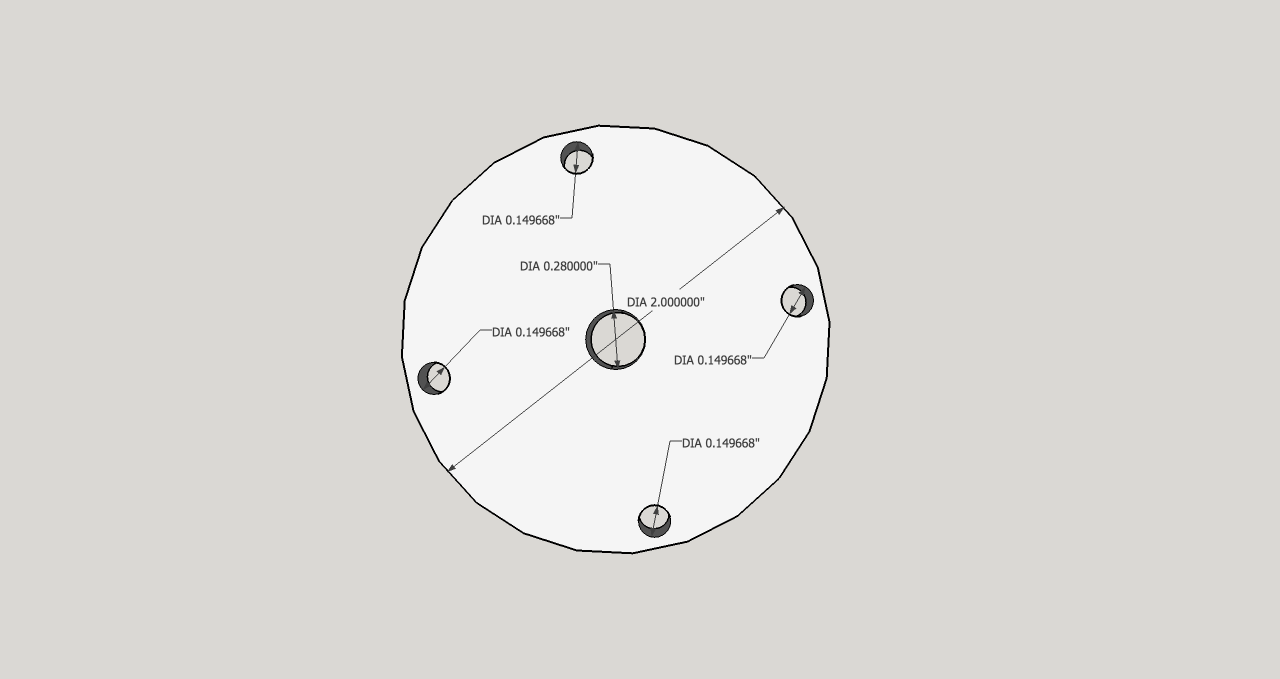
\includegraphics[width=\textwidth]{./mechanical/PZT_holder_bottom.png}
	\caption[Cavity Mounts]{The bottom up view and measurements of the PZT-Mirror holder}
	\label{fig:PZT-holder-bottom}
\end{figure}  

\begin{figure}[h!]
  \centering
	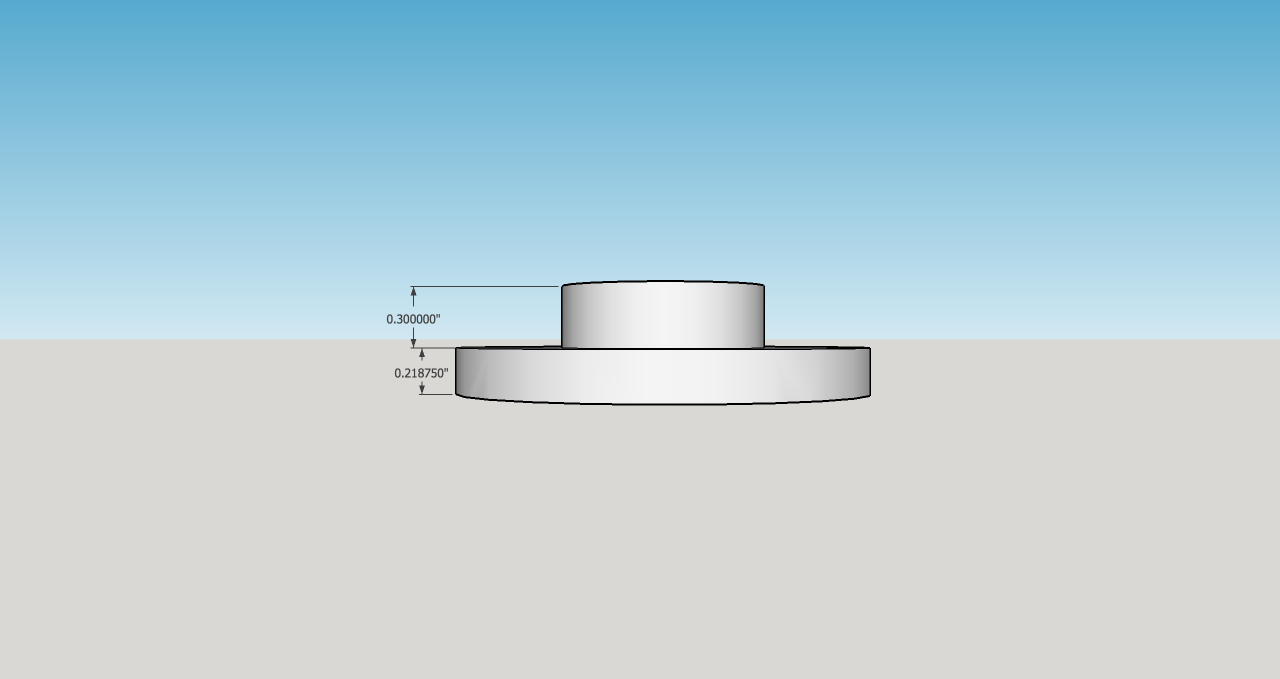
\includegraphics[width=\textwidth]{./mechanical/PZT_holder_side.png}
	\caption[Cavity Mounts]{The side view and measurements of the PZT-Mirror holder}
	\label{fig:PZT-holder-side}
\end{figure}  

\newpage

\subsection{sFPI Aluminum Base} \label{ss:sfpilensholder}

\begin{figure}[h!]
  \centering
	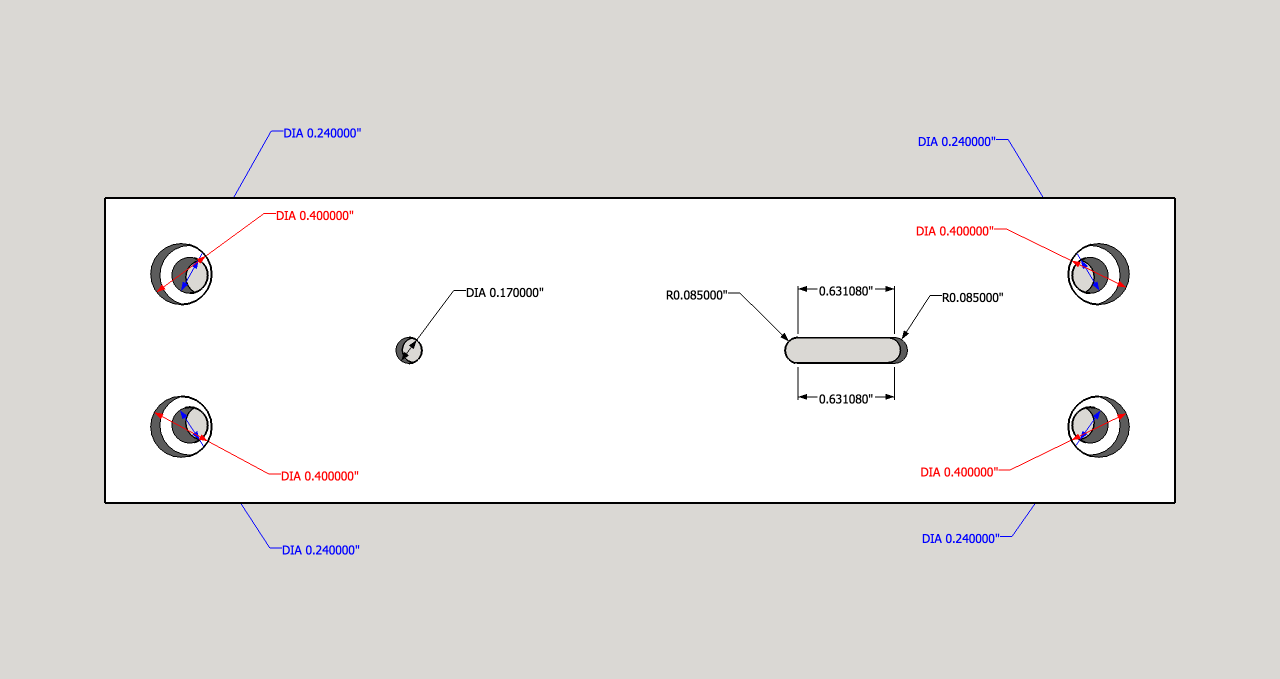
\includegraphics[width=\textwidth]{./mechanical/sfpilensholder_top.png}
	\caption[Cavity Mounts]{The top down view and measurements of the sFPI aluminum base}
	\label{fig:sfpilensholder-top}
\end{figure}  

\begin{figure}[h!]
  \centering
	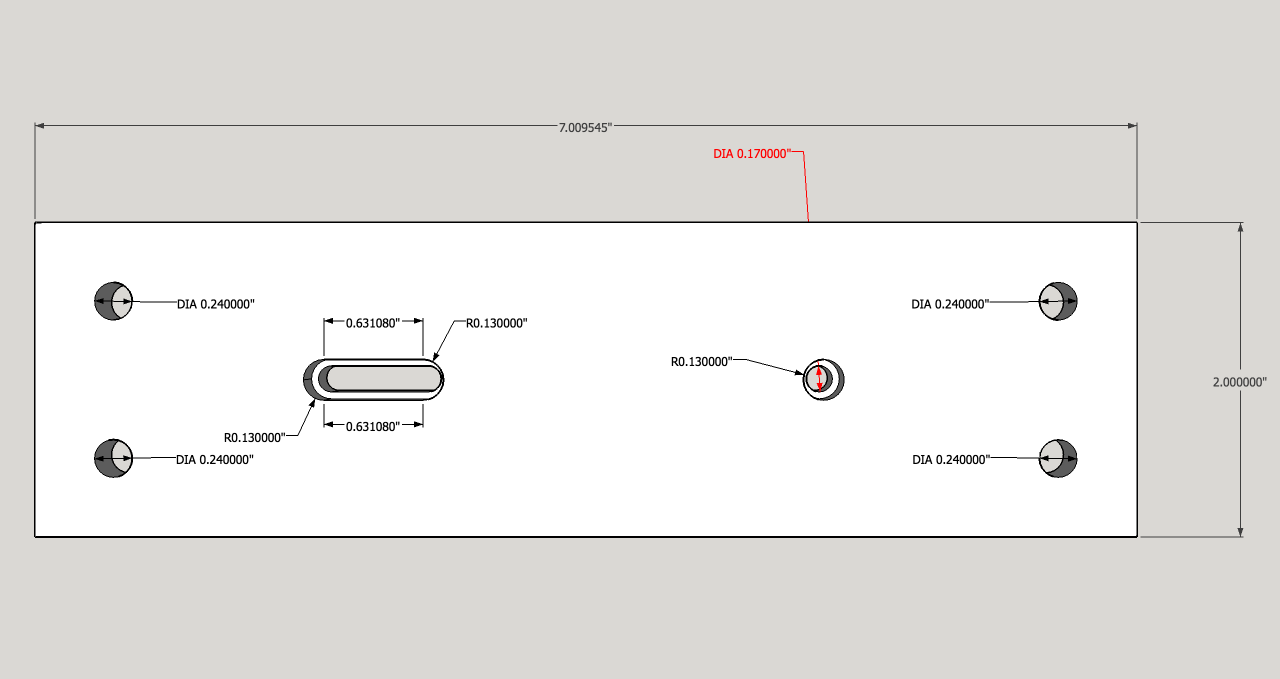
\includegraphics[width=\textwidth]{./mechanical/sfpilensholder_bottom.png}
	\caption[Cavity Mounts]{The bottom up view and measurements of the sFPI aluminum base}
	\label{fig:sfpilensholder-bottom}
\end{figure}  

\begin{figure}[h!]
  \centering
	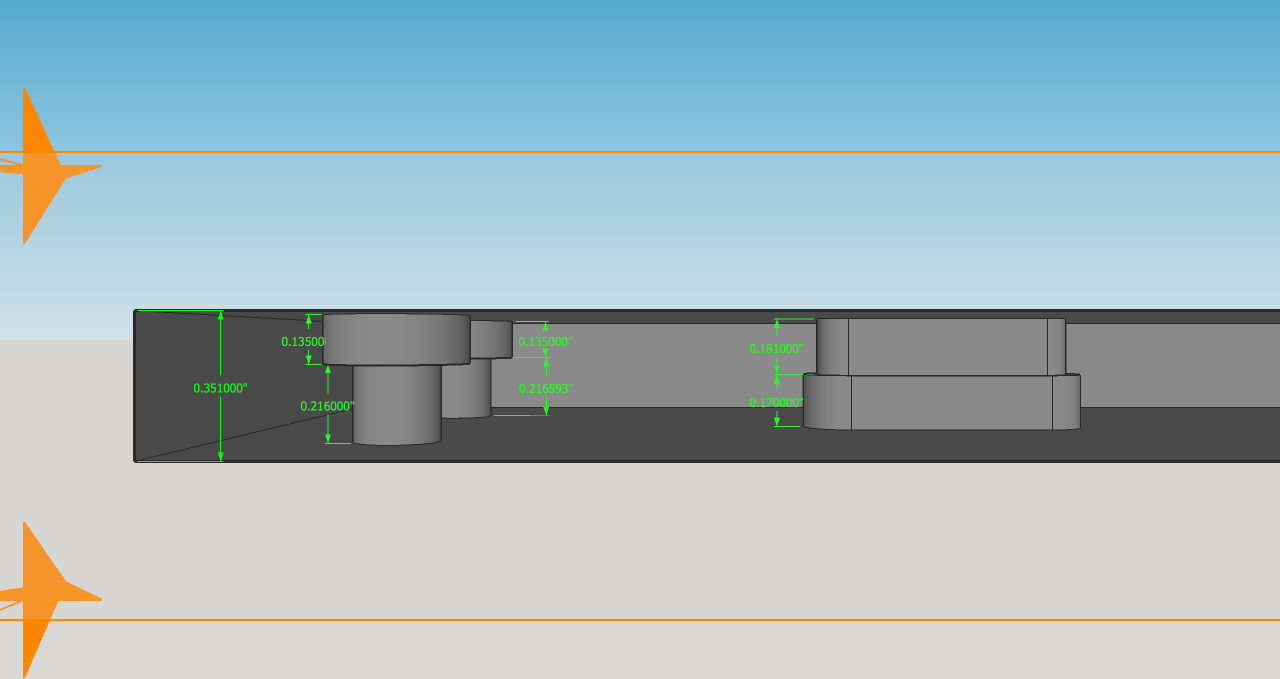
\includegraphics[width=\textwidth]{./mechanical/sfpilensholder_cross_section_1.png}
	\caption[Cavity Mounts]{The front cross section view and measurements of the sFPI aluminum base}
	\label{fig:sfpilensholder-side}
\end{figure} 

\begin{figure}[h!]
  \centering
	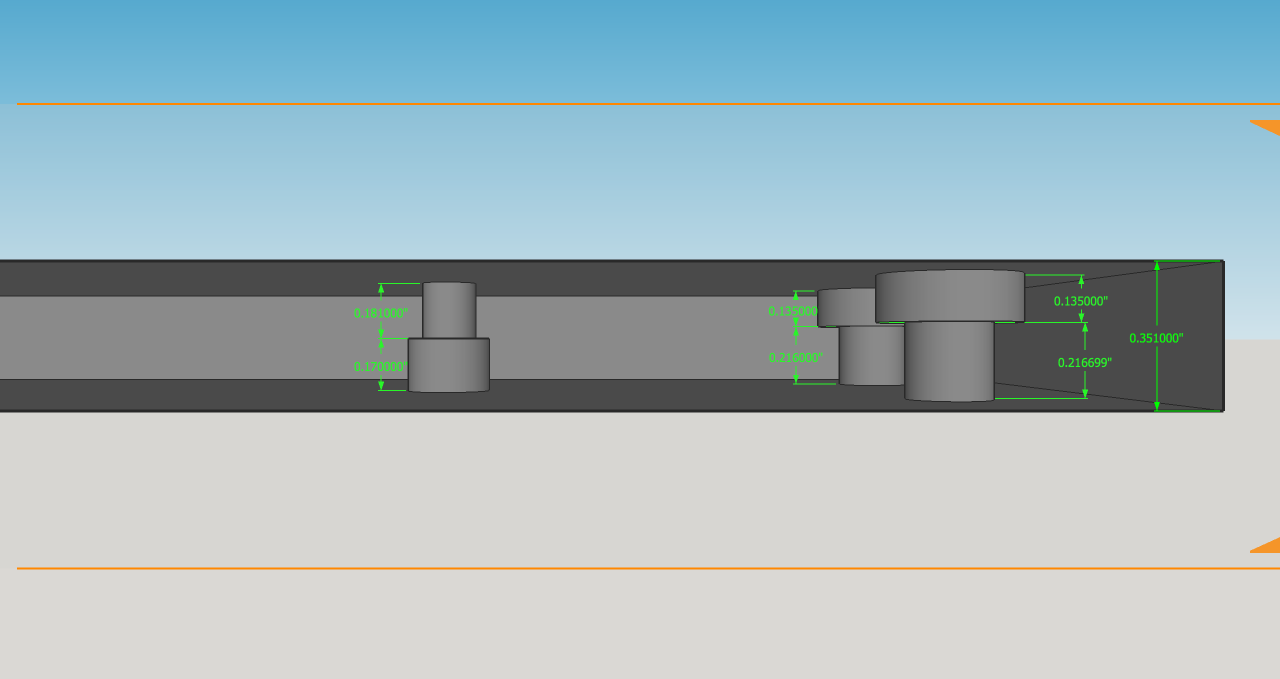
\includegraphics[width=\textwidth]{./mechanical/sfpilensholder_cross_section_2.png}
	\caption[Cavity Mounts]{The back cross section view and measurements of the sFPI aluminum base}
	\label{fig:sfpilensholder-side}
\end{figure}   

\newpage

\subsection{Photodiode Holder} \label{ss:diode_holder}

\begin{figure}[h!]
  \centering
	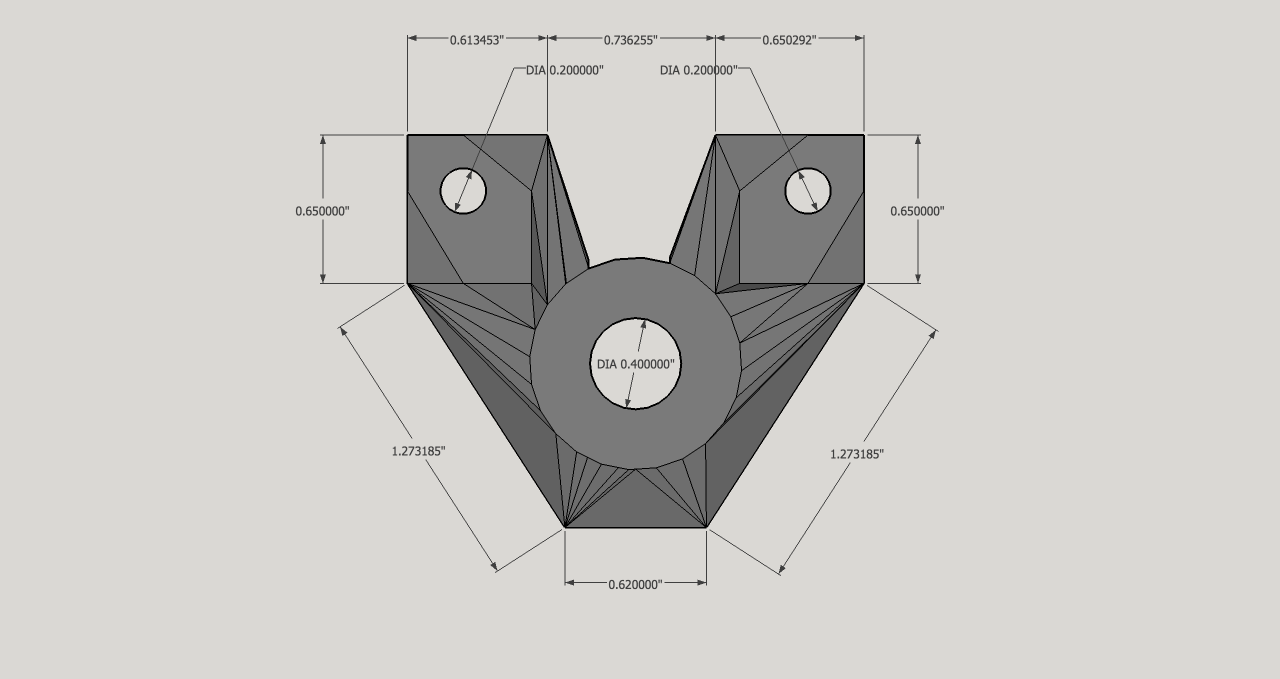
\includegraphics[width=\textwidth]{./mechanical/diode_holder_top.png}
	\caption[Cavity Mounts]{The top down view and measurements of the sFPI aluminum base}
	\label{fig:diode_holder-top}
\end{figure}  

\begin{figure}[h!]
  \centering
	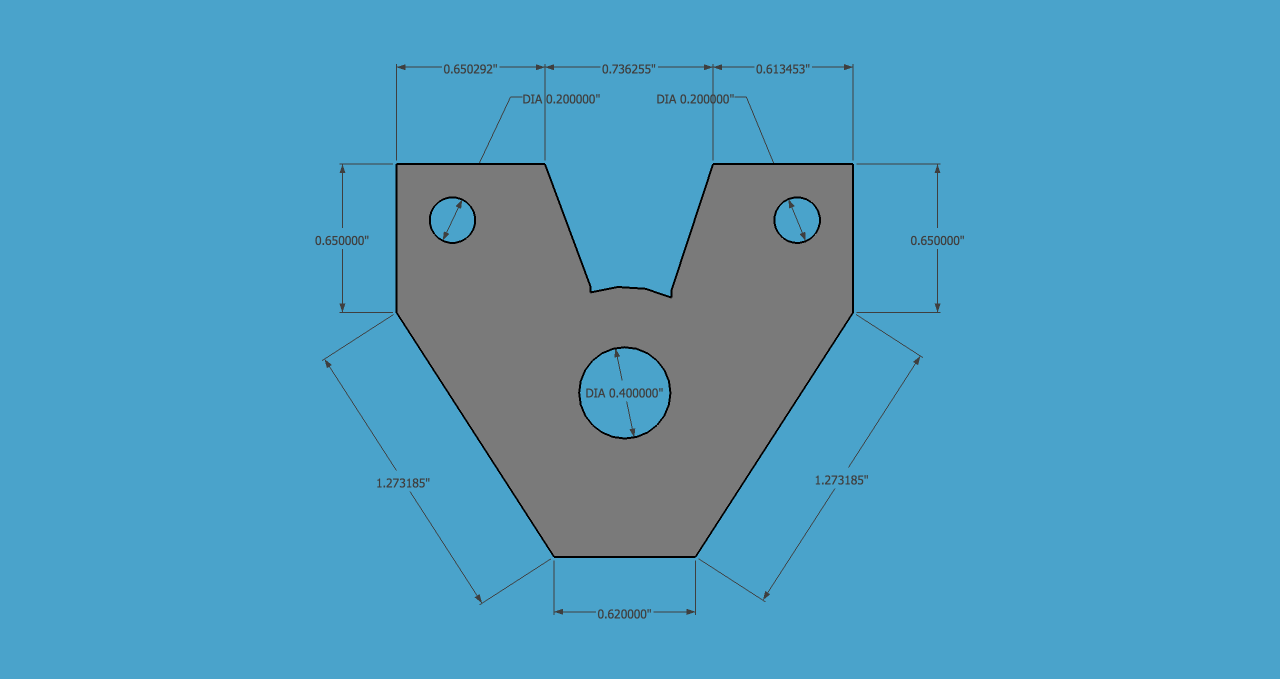
\includegraphics[width=\textwidth]{./mechanical/diode_holder_bottom.png}
	\caption[Cavity Mounts]{The bottom up view and measurements of the sFPI aluminum base}
	\label{fig:diode_holder-bottom}
\end{figure}  

\begin{figure}[h!]
  \centering
	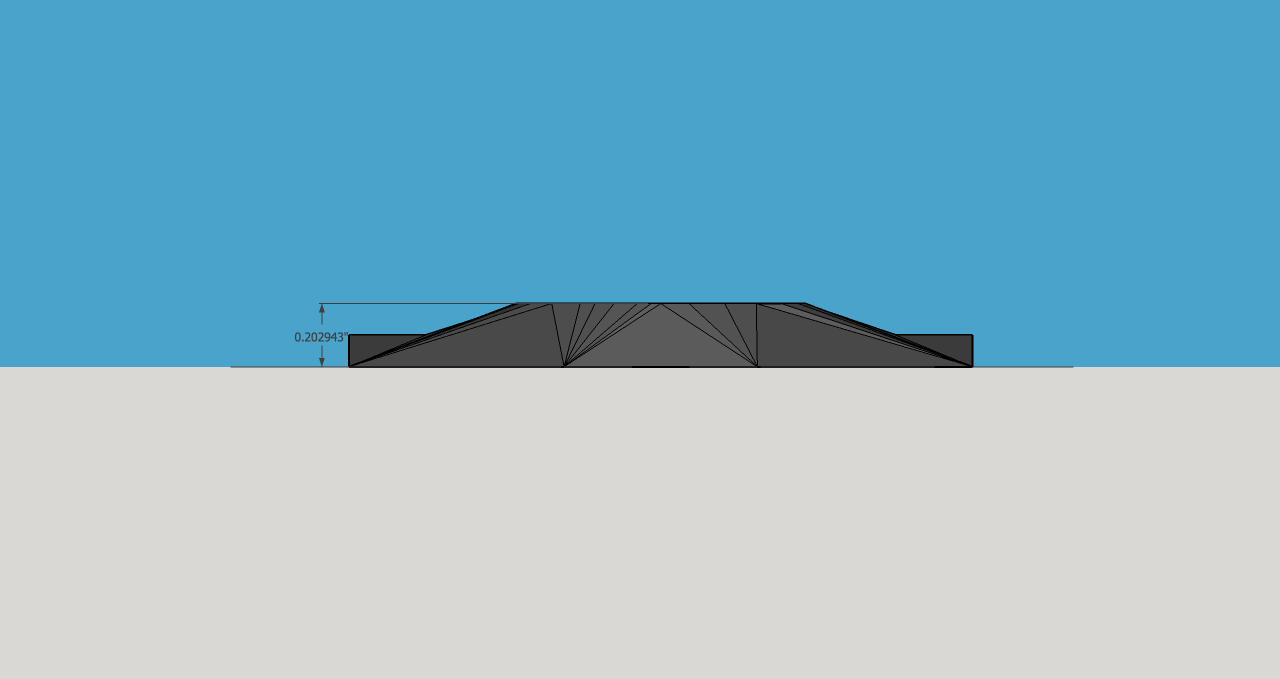
\includegraphics[width=\textwidth]{./mechanical/diode_holder_front.png}
	\caption[Cavity Mounts]{The front cross section view and measurements of the sFPI aluminum base}
	\label{fig:diode_holder-front}
\end{figure} 

\begin{figure}[h!]
  \centering
	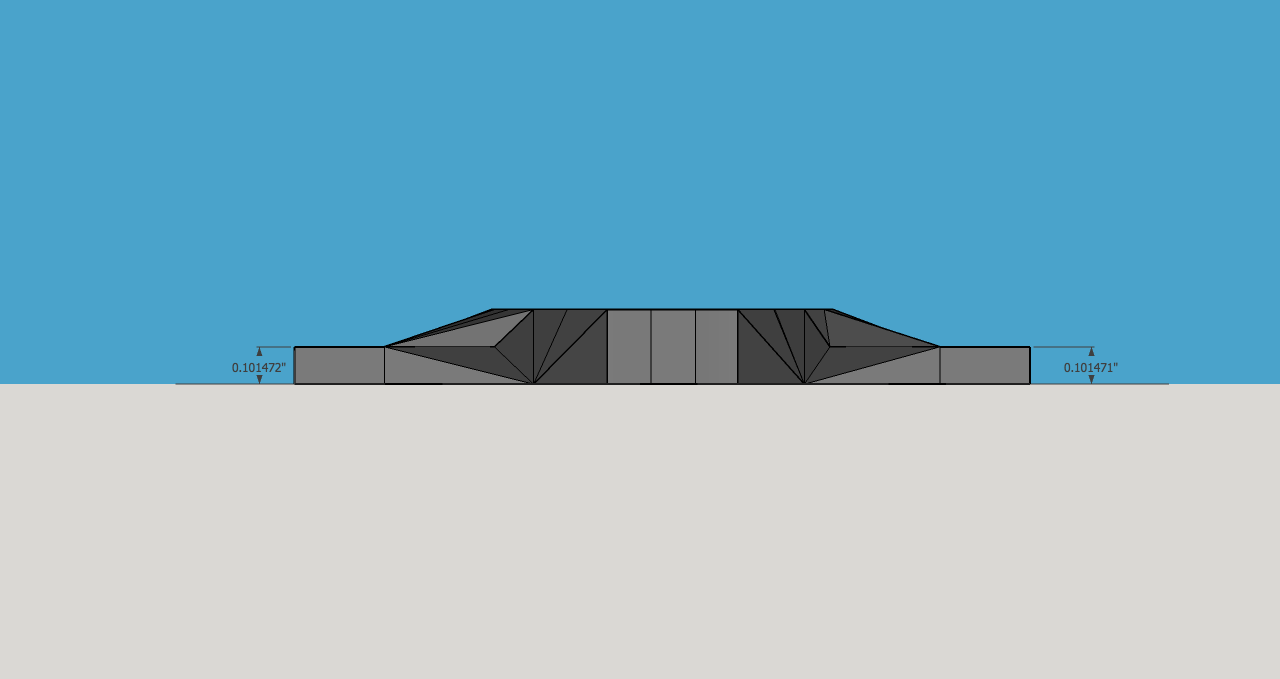
\includegraphics[width=\textwidth]{./mechanical/diode_holder_back.png}
	\caption[Cavity Mounts]{The back cross section view and measurements of the sFPI aluminum base}
	\label{fig:diode_holder-back}
\end{figure}  

\begin{figure}[h!]
  \centering
	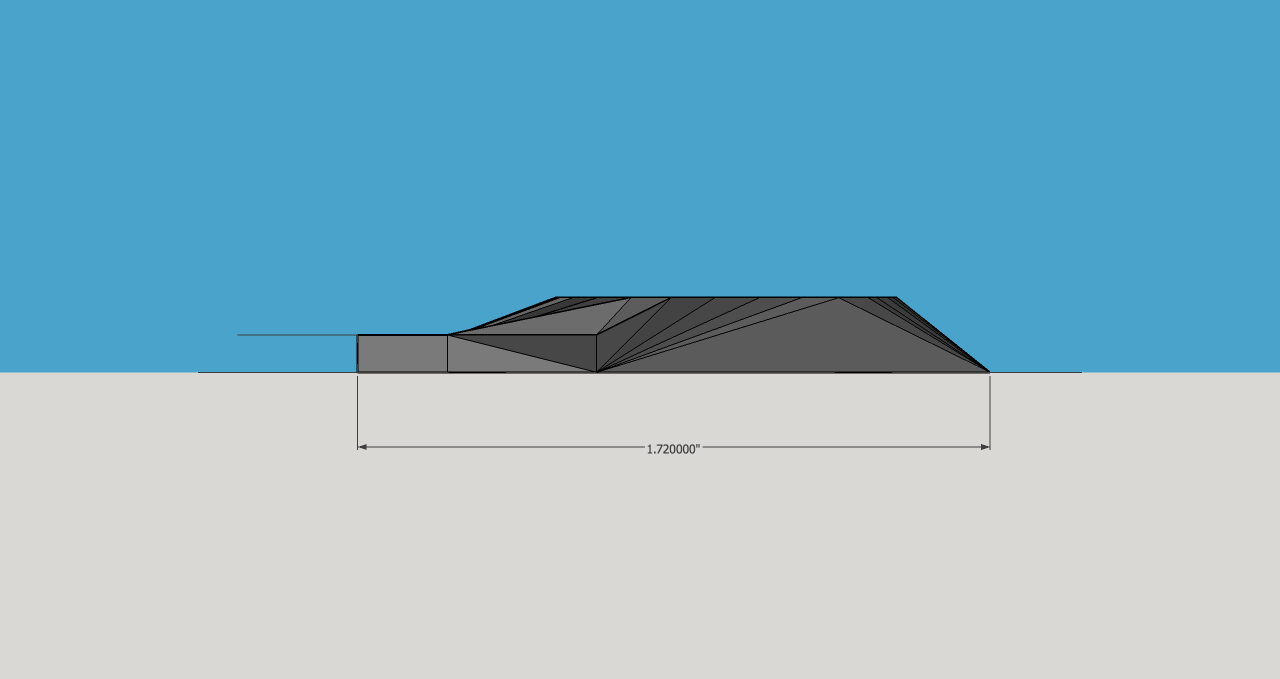
\includegraphics[width=\textwidth]{./mechanical/diode_holder_side.png}
	\caption[Cavity Mounts]{The back cross section view and measurements of the sFPI aluminum base}
	\label{fig:diode_holder-side}
\end{figure}   

\newpage

\section{Arduino Programs}
\subsection{Writing to the MCP4725 12-bit DAC via I2C}
\arduinoexternal{../App/Arduino/sFPI-driver/sFPI-driver.ino}

\subsection{Program for capturing and sending serial data to the computer} \label{serial-data}
\arduinoexternal{../App/Arduino/Serial-data/Serial-data.ino}

\section{Python GUI}

\subsection{Main program}
\pythonexternal{../App/GUI.py}

\subsection{Application Class}
\pythonexternal{../App/Application.py}

\subsection{USB Interface Class}
\pythonexternal{../App/USBInterface.py}

\subsection{GUI Errors Class}
\pythonexternal{../App/GUIErrors.py}

\subsection{Setup Function}
\pythonexternal{../App/setup.py}
\newpage

\section{LTSpice Netlists}
\subsection{Interferometer Driver LTSpice Netlist for Simulation}
\ltspiceexternal{../Electrical_Design/Amplifier_Design/amplifier_setup_rev2.txt}
\newpage

\section{Schematics}

\begin{figure}[h!]
	\centering
	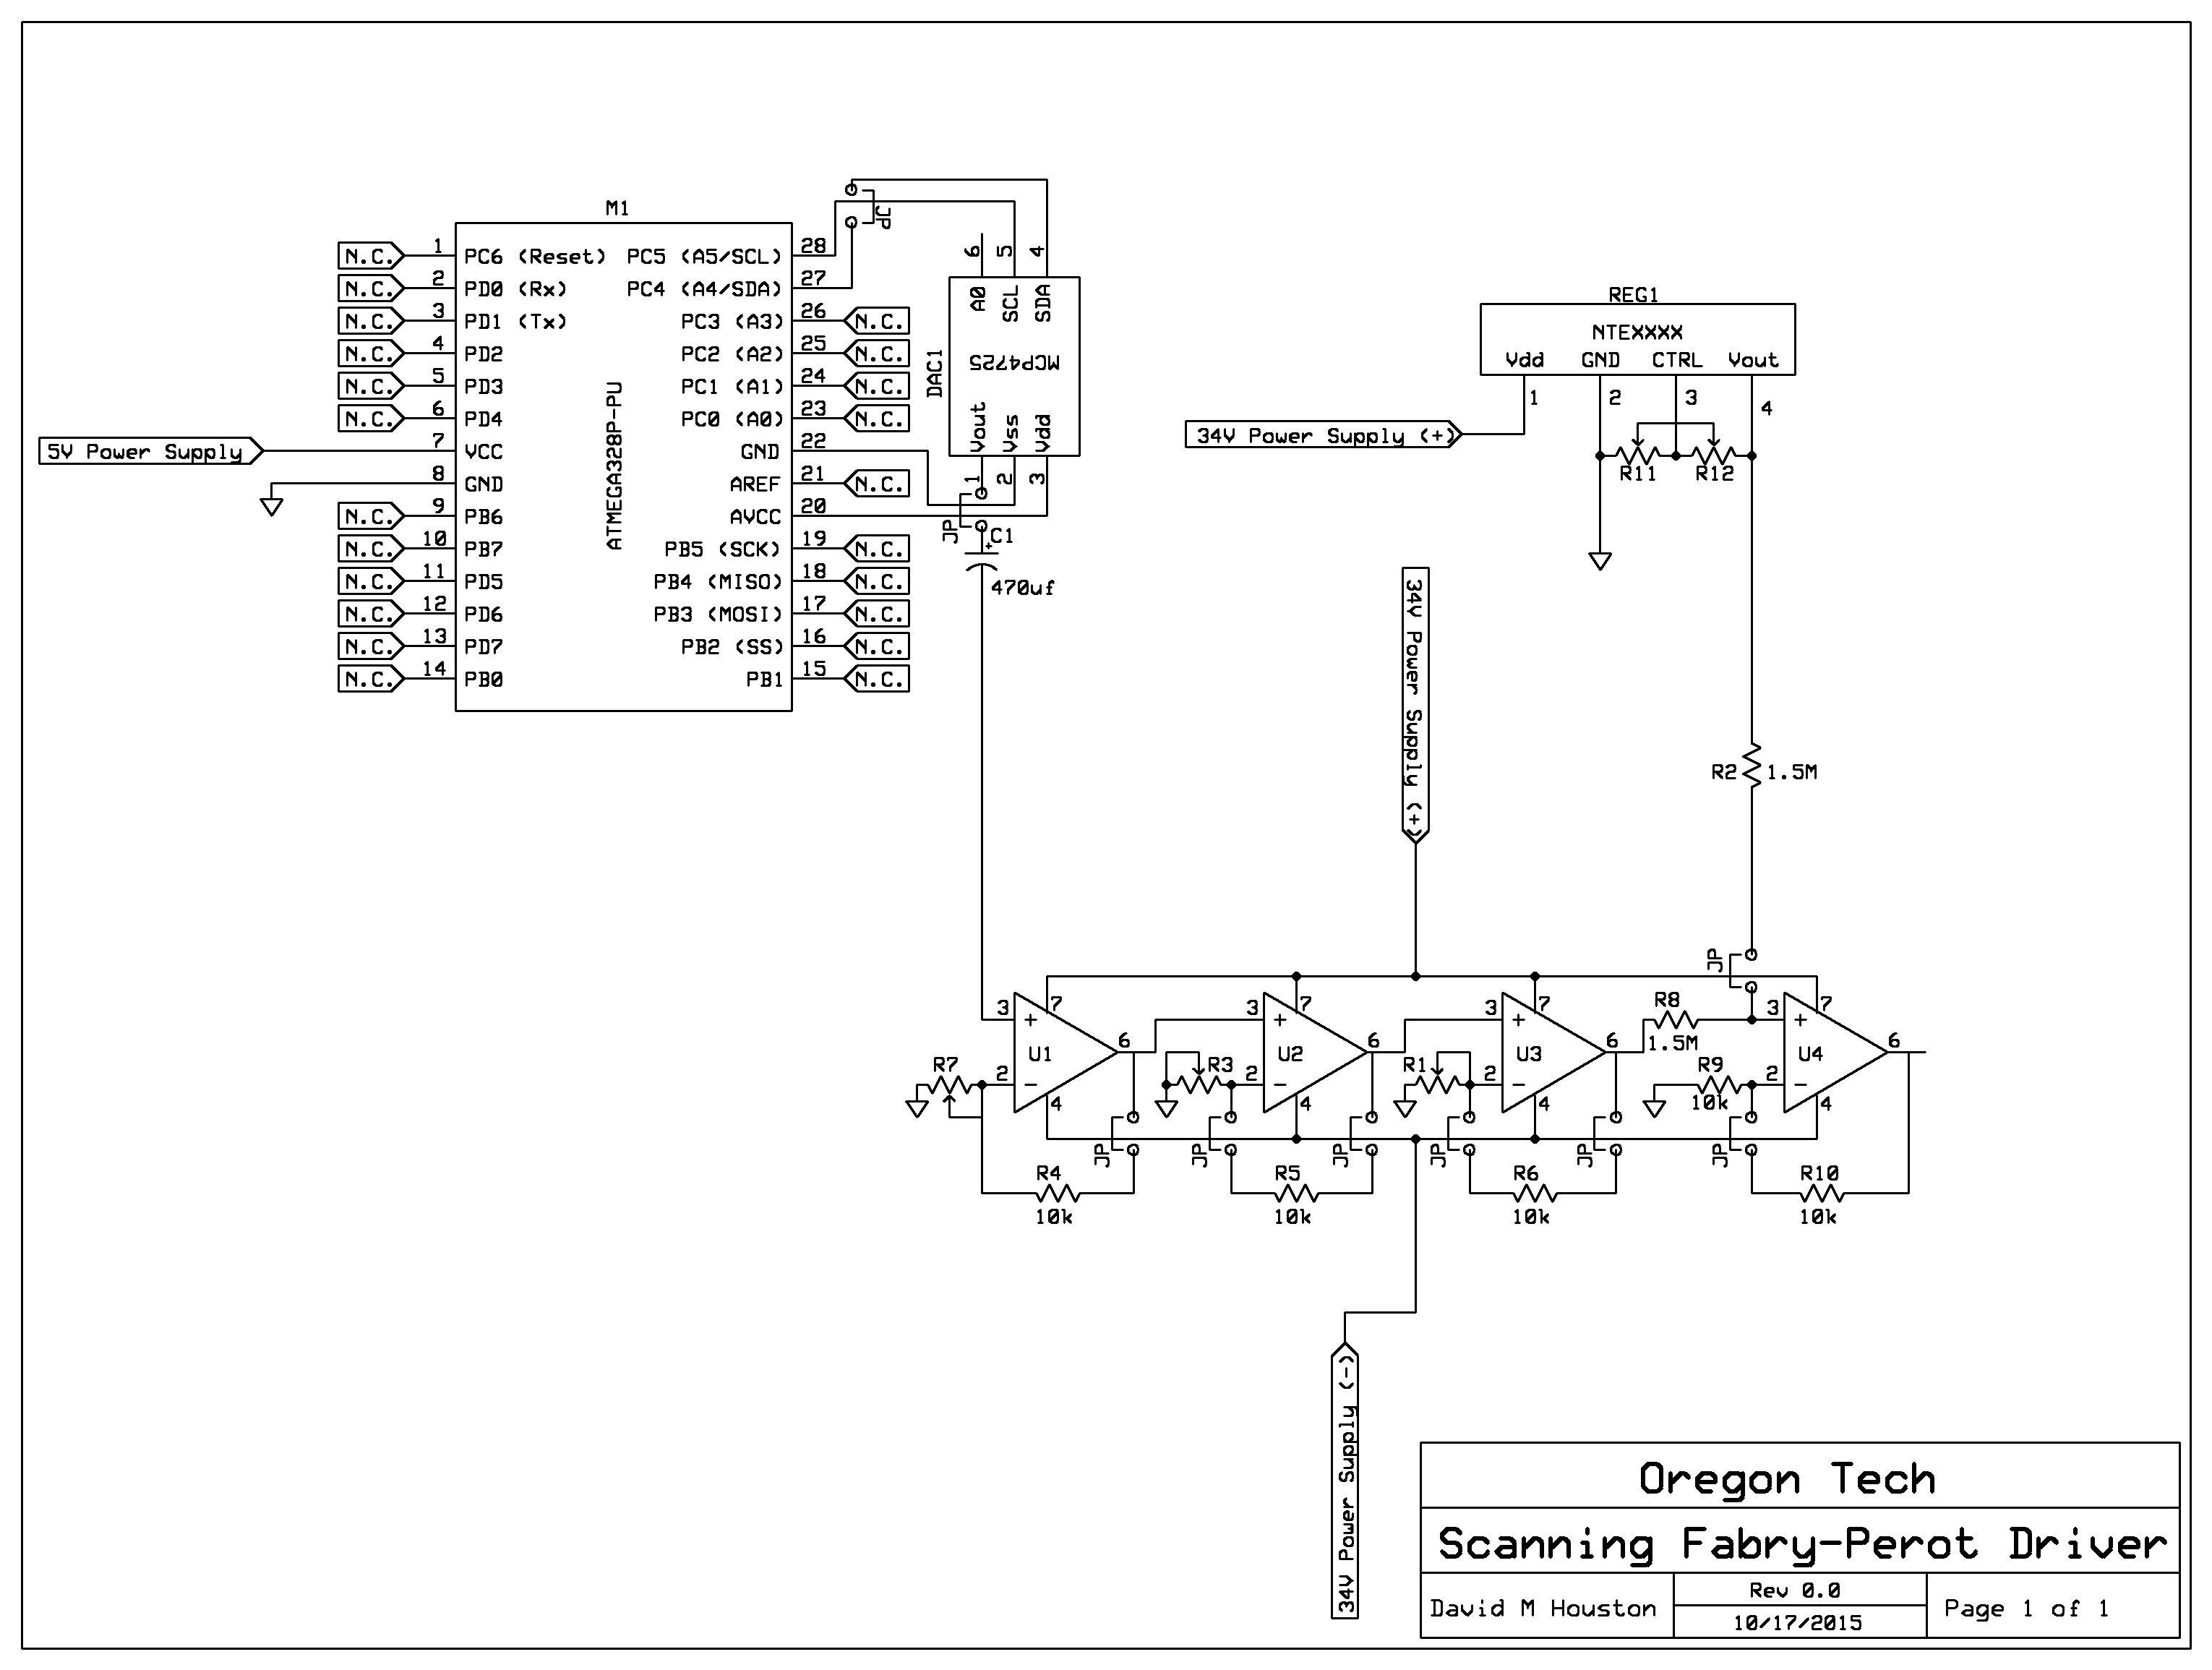
\includegraphics[width=\textwidth]{schematic-driver.png}
	\caption[Block Diagram]{Driver Schematic}
	\label{schm:driver-schematic}
\end{figure}
\newpage
\begin{figure}[h!]
	\centering
	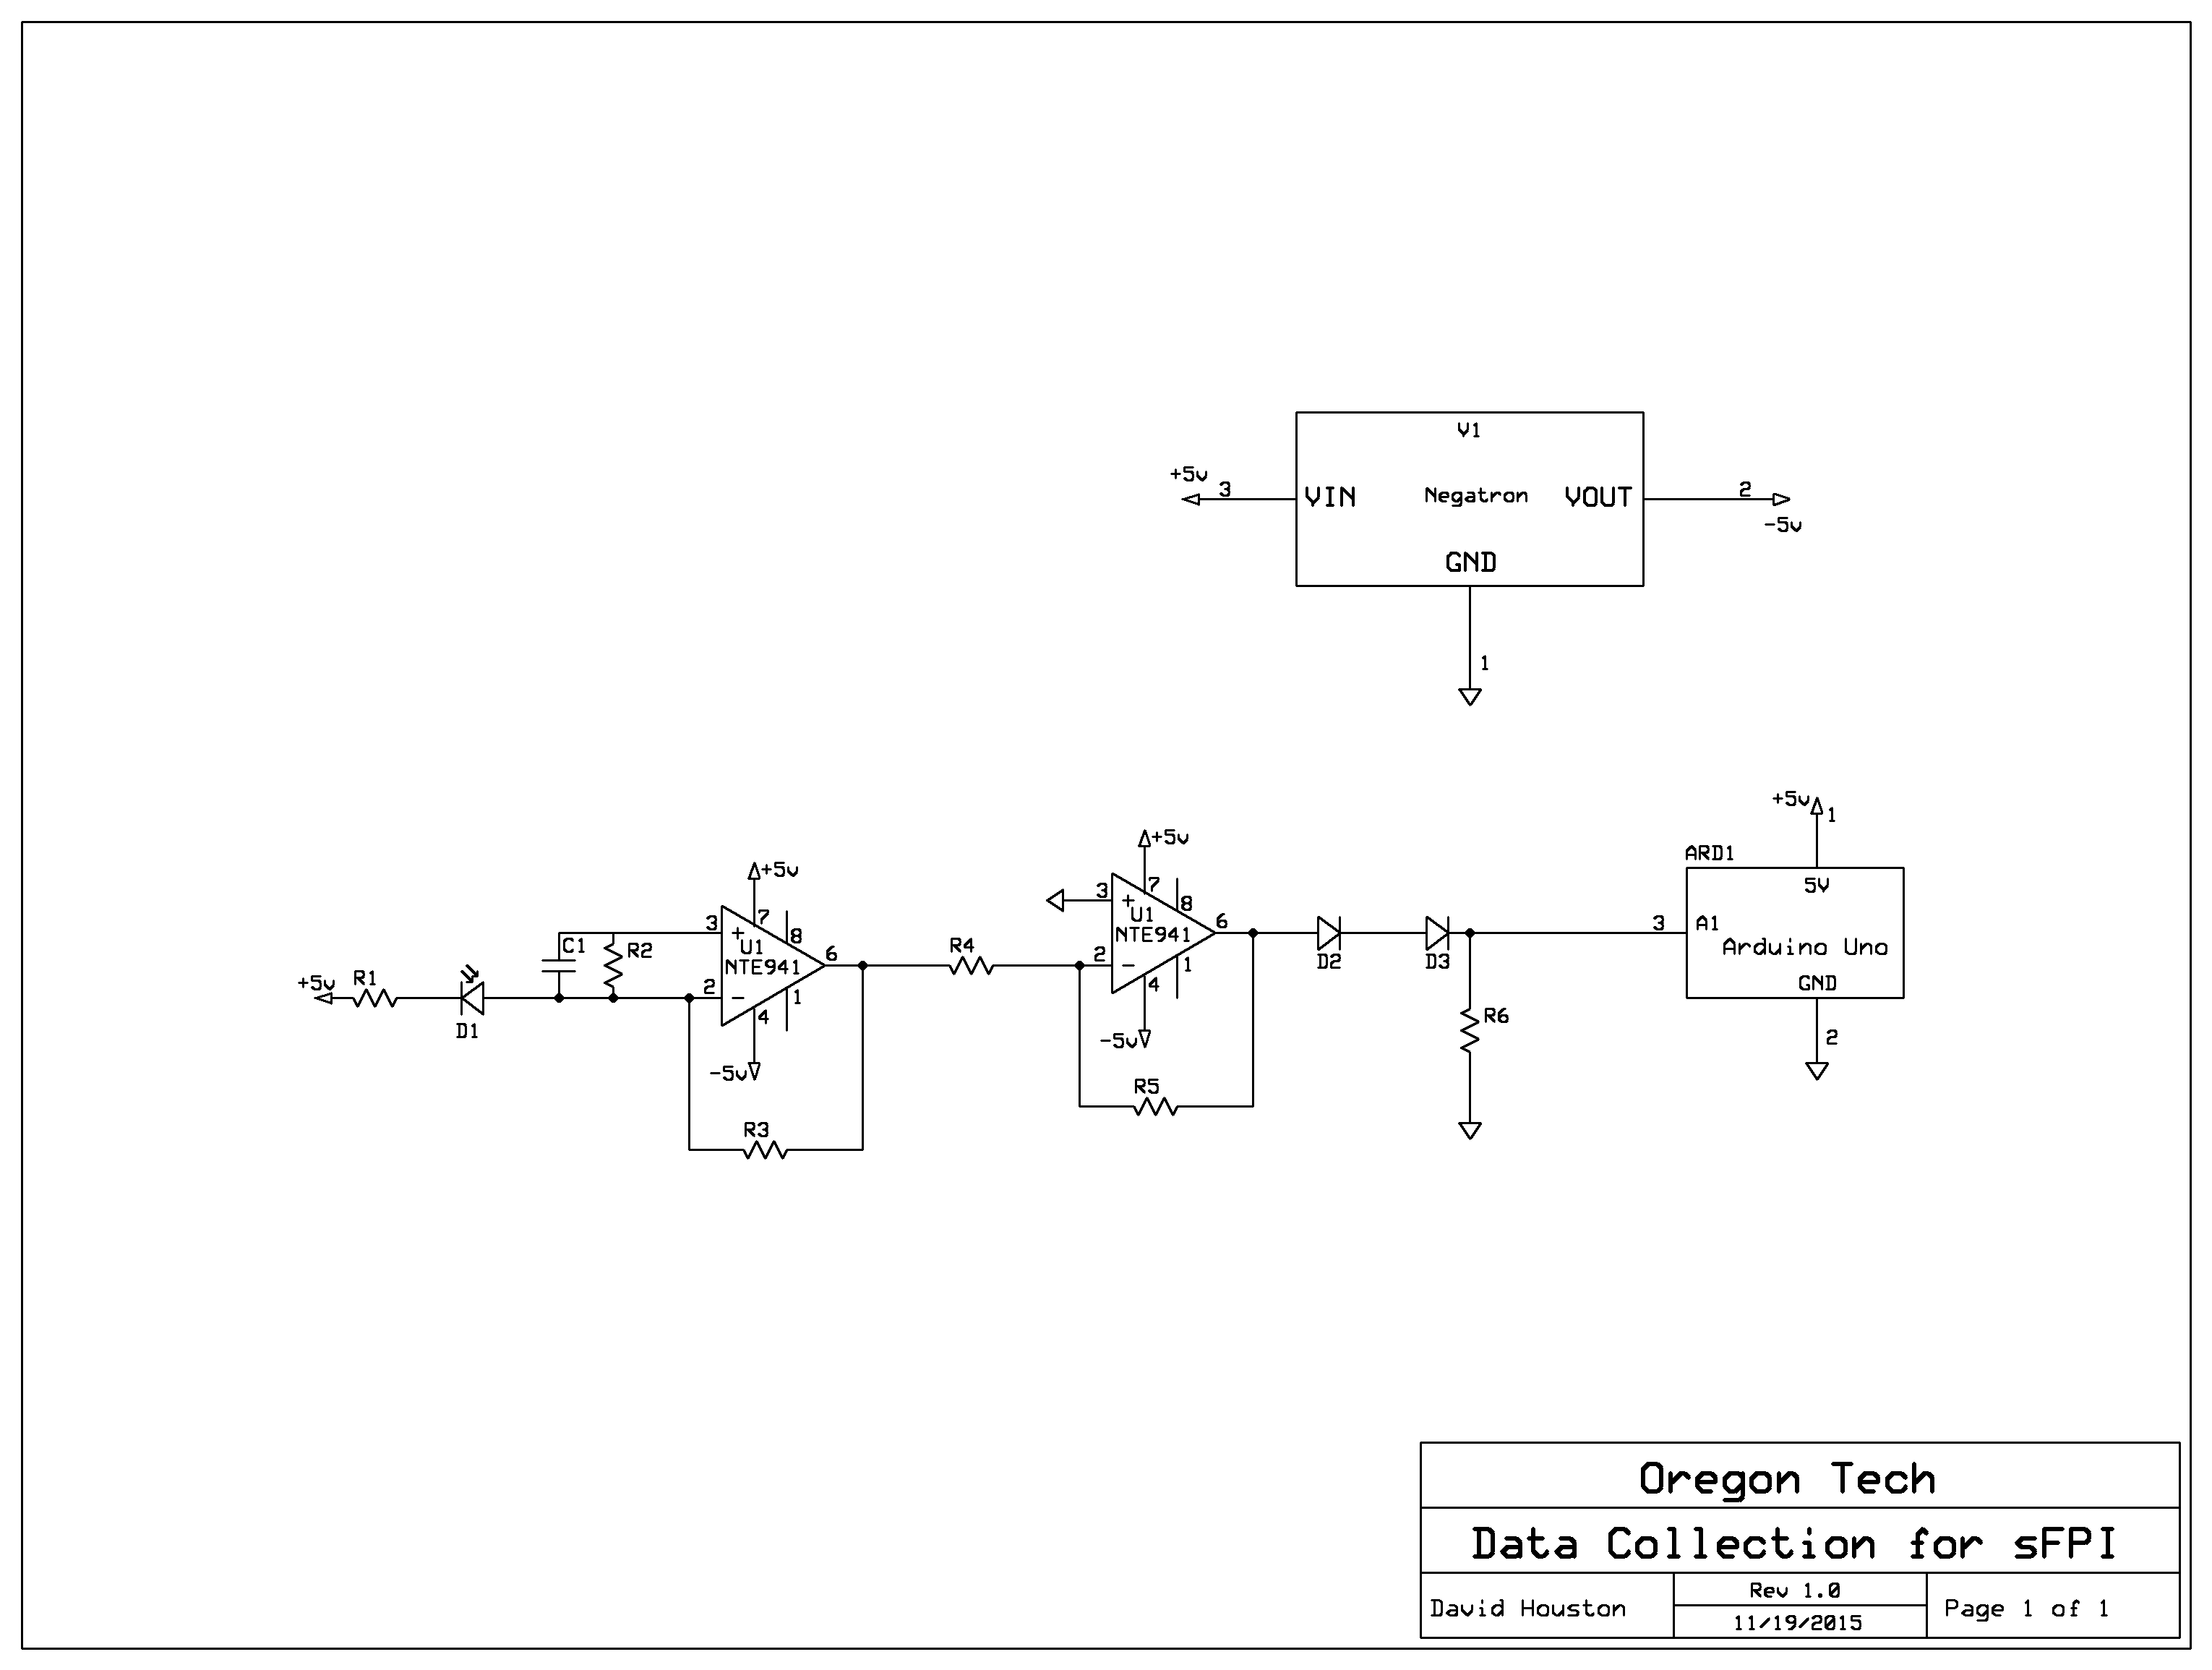
\includegraphics[width=\textwidth]{schematic-photodiode.png}
	\caption[Photodiode Output Circuit]{Reverse Biased Transimpedance Amplifier of the Photodiode output}
	\label{schm:photodiode}
\end{figure}
\newpage
\begin{figure}[h!]
	\centering
	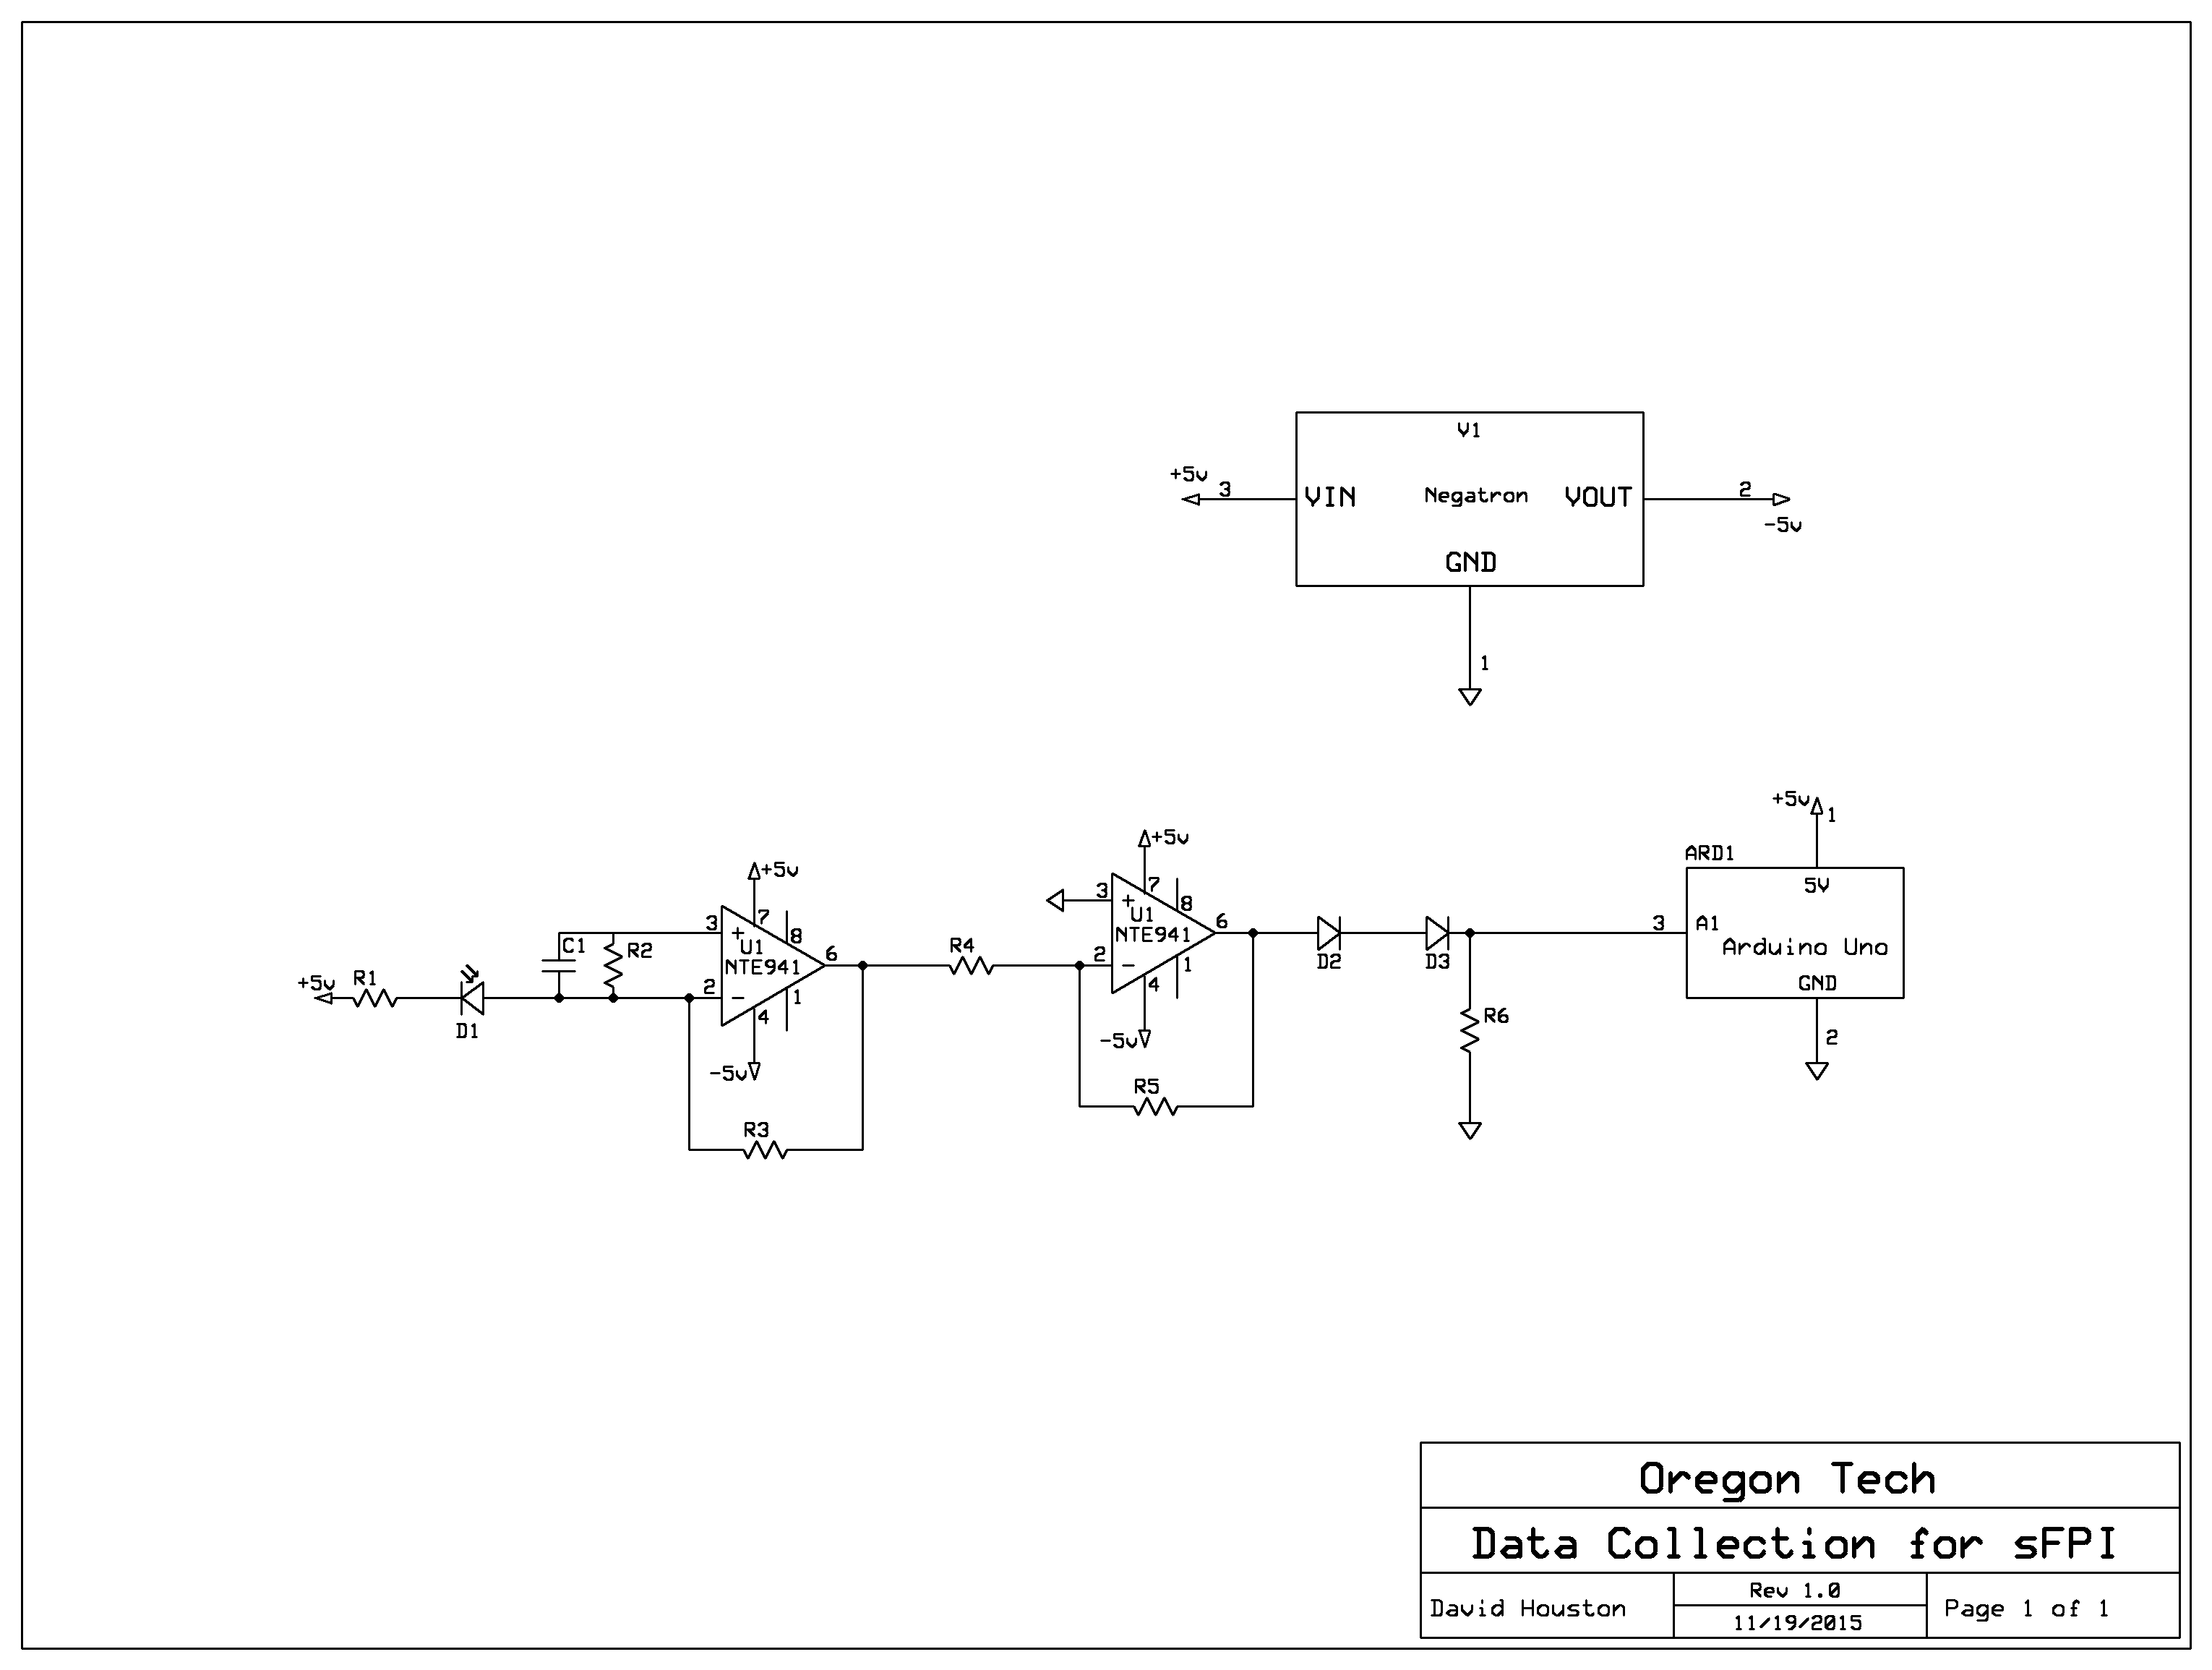
\includegraphics[width=\textwidth]{schematic-power.png}
	\caption[Photodiode Output Circuit]{Power Distribution Schematic}
	\label{schm:power-distribution}
\end{figure}
\newpage

\section{LTSpice Models} \label{ss:ltpsice-models}

\begin{figure}[h!]
	\centering
	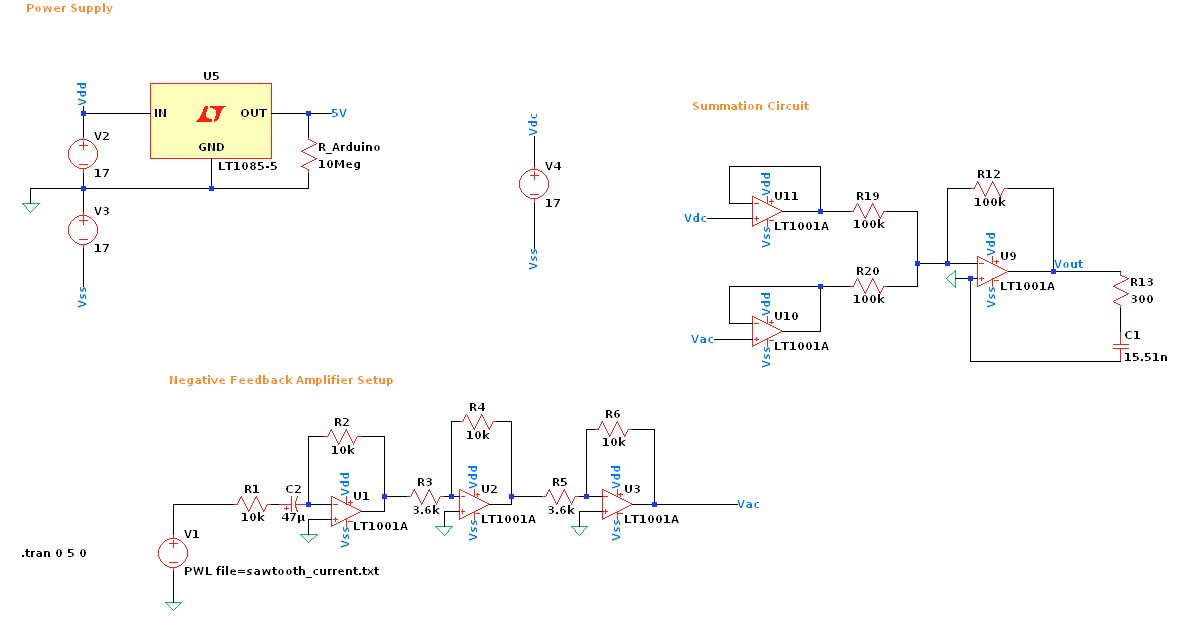
\includegraphics[width=\textwidth]{/ltspice/driver-ltspice-model.png}
	\caption{LTSpice Model for sFPI electrical driver design}
	\label{ltpsice:driver}
\end{figure}

\newpage

\section{Datasheets}

%\includepdf[pages=1-15]{./datasheets/ATmega328.pdf}

%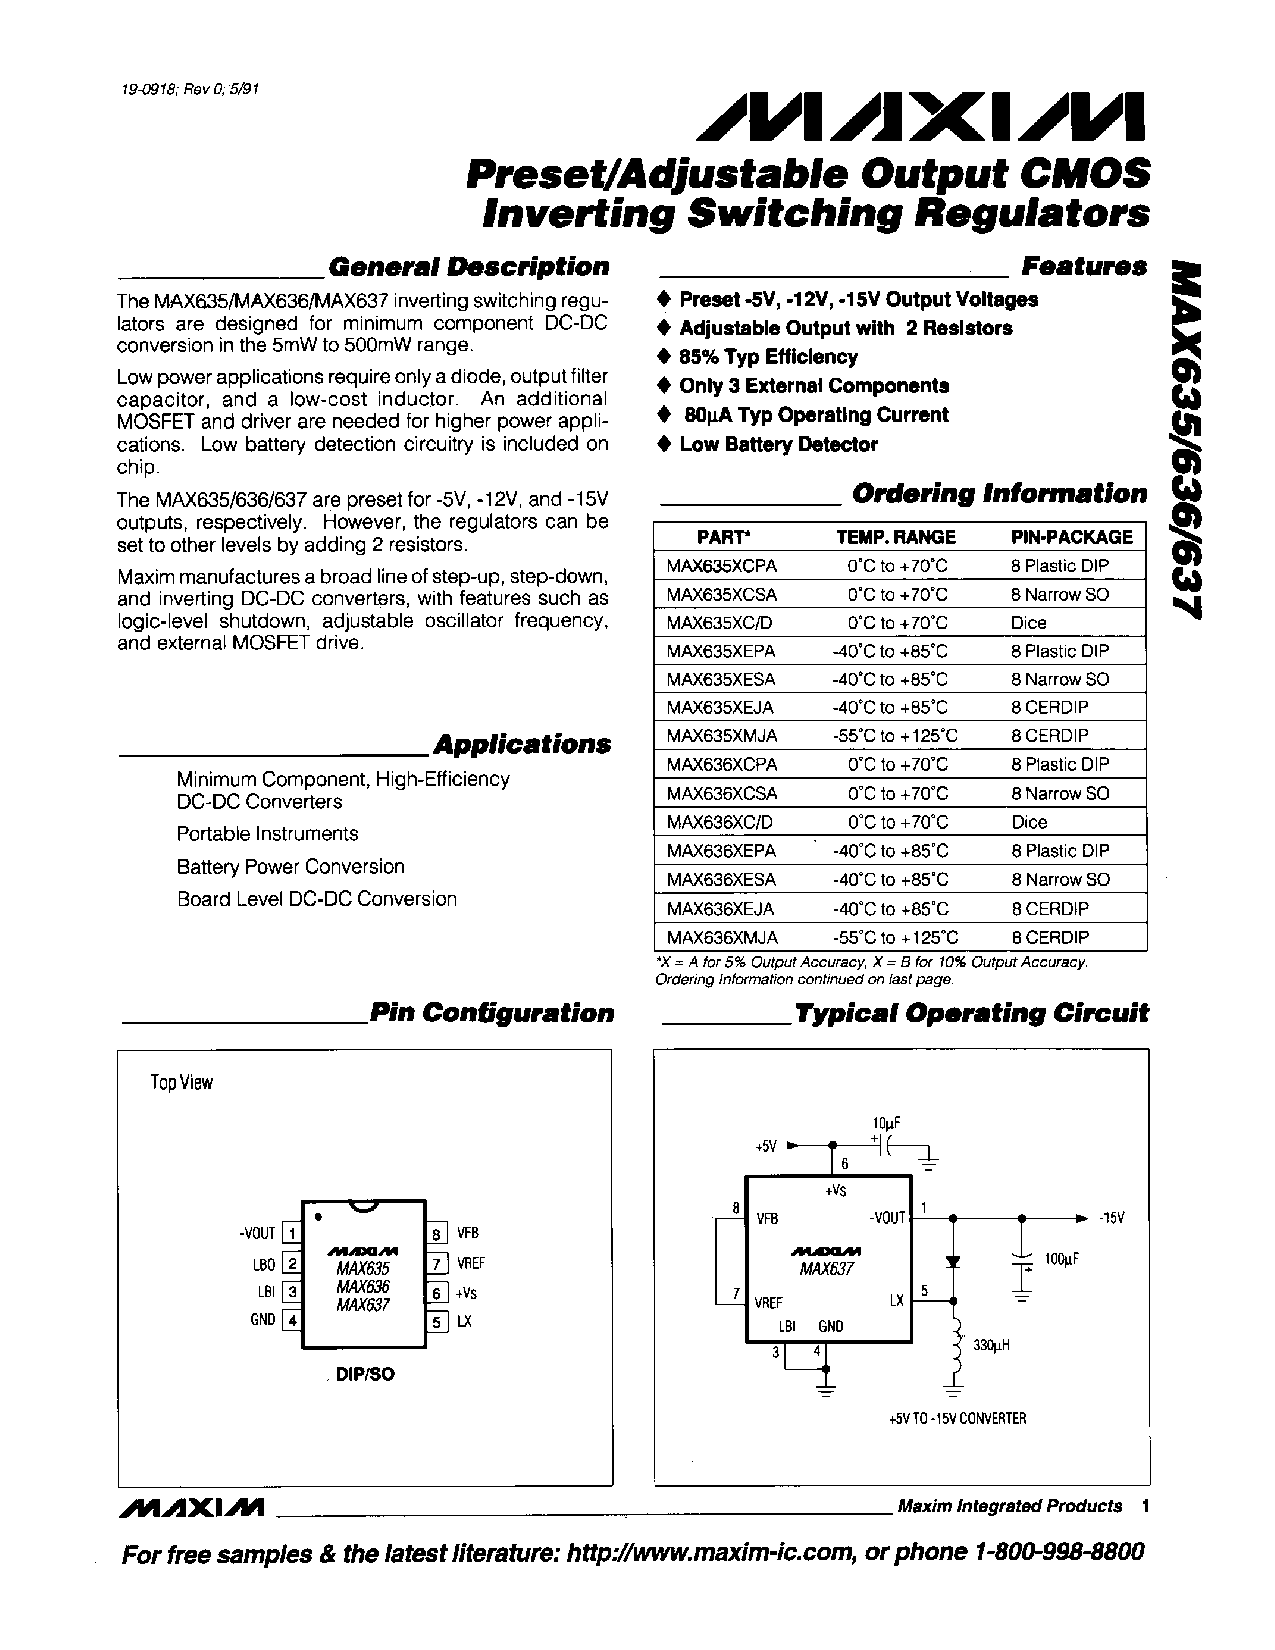
\includepdf[pages=-]{./datasheets/MAX635.pdf}

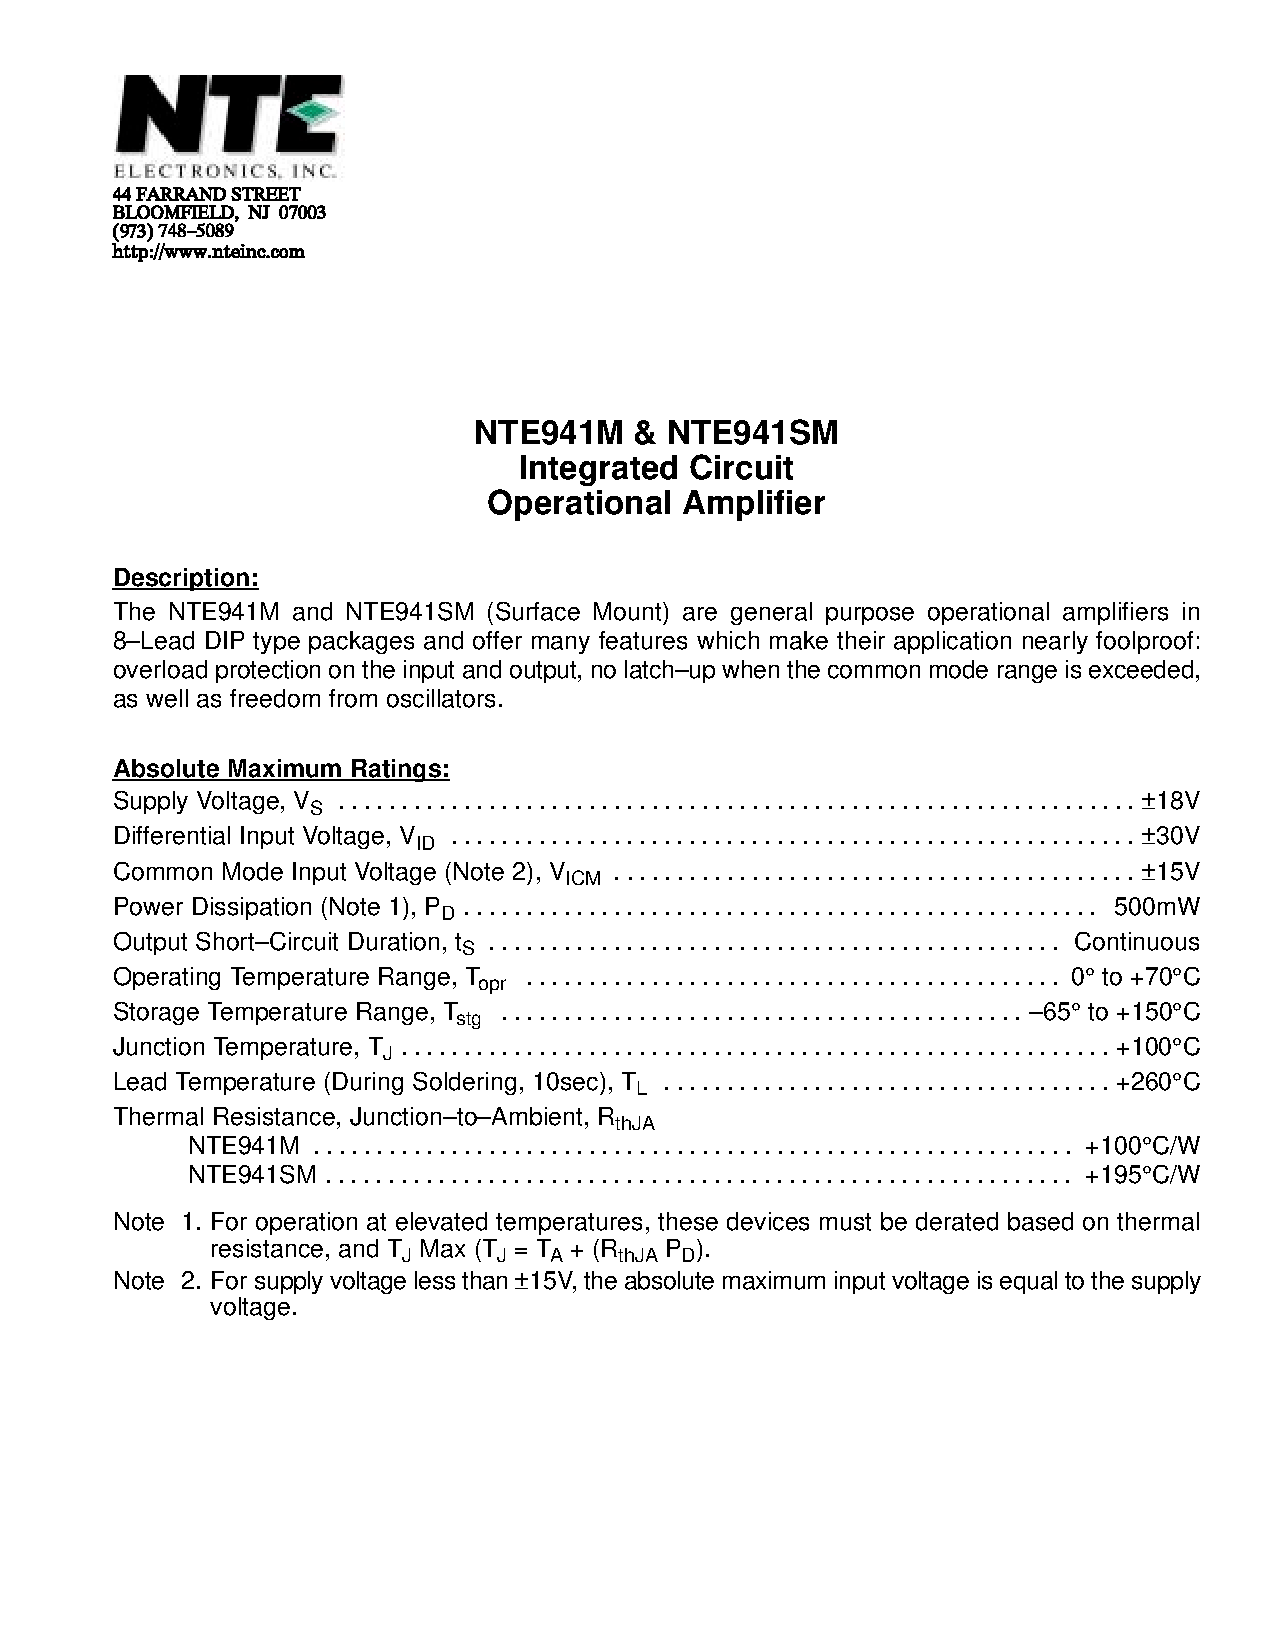
\includepdf[pages=-]{./datasheets/nte941m.pdf} \label{datasheet:nte941m}

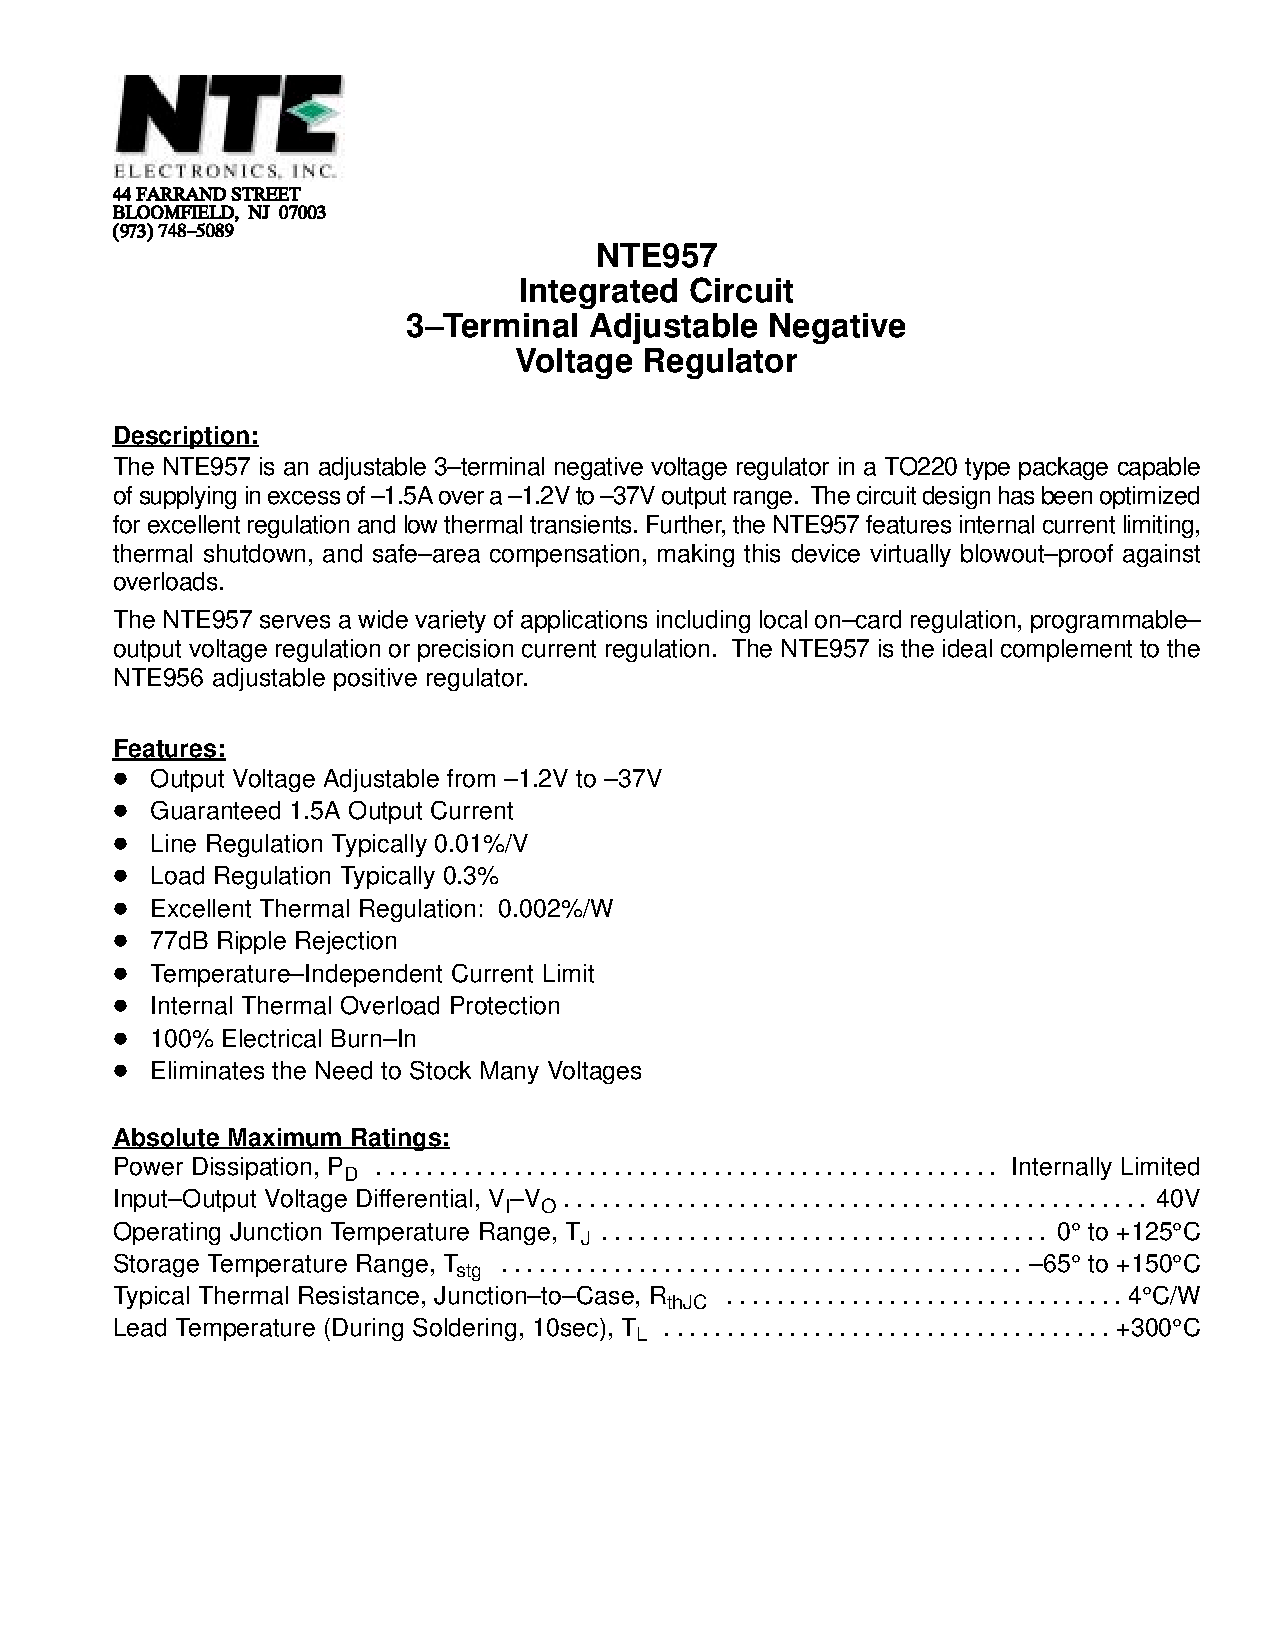
\includepdf[pages=-]{./datasheets/nte957.pdf} \label{datasheet:nte957}

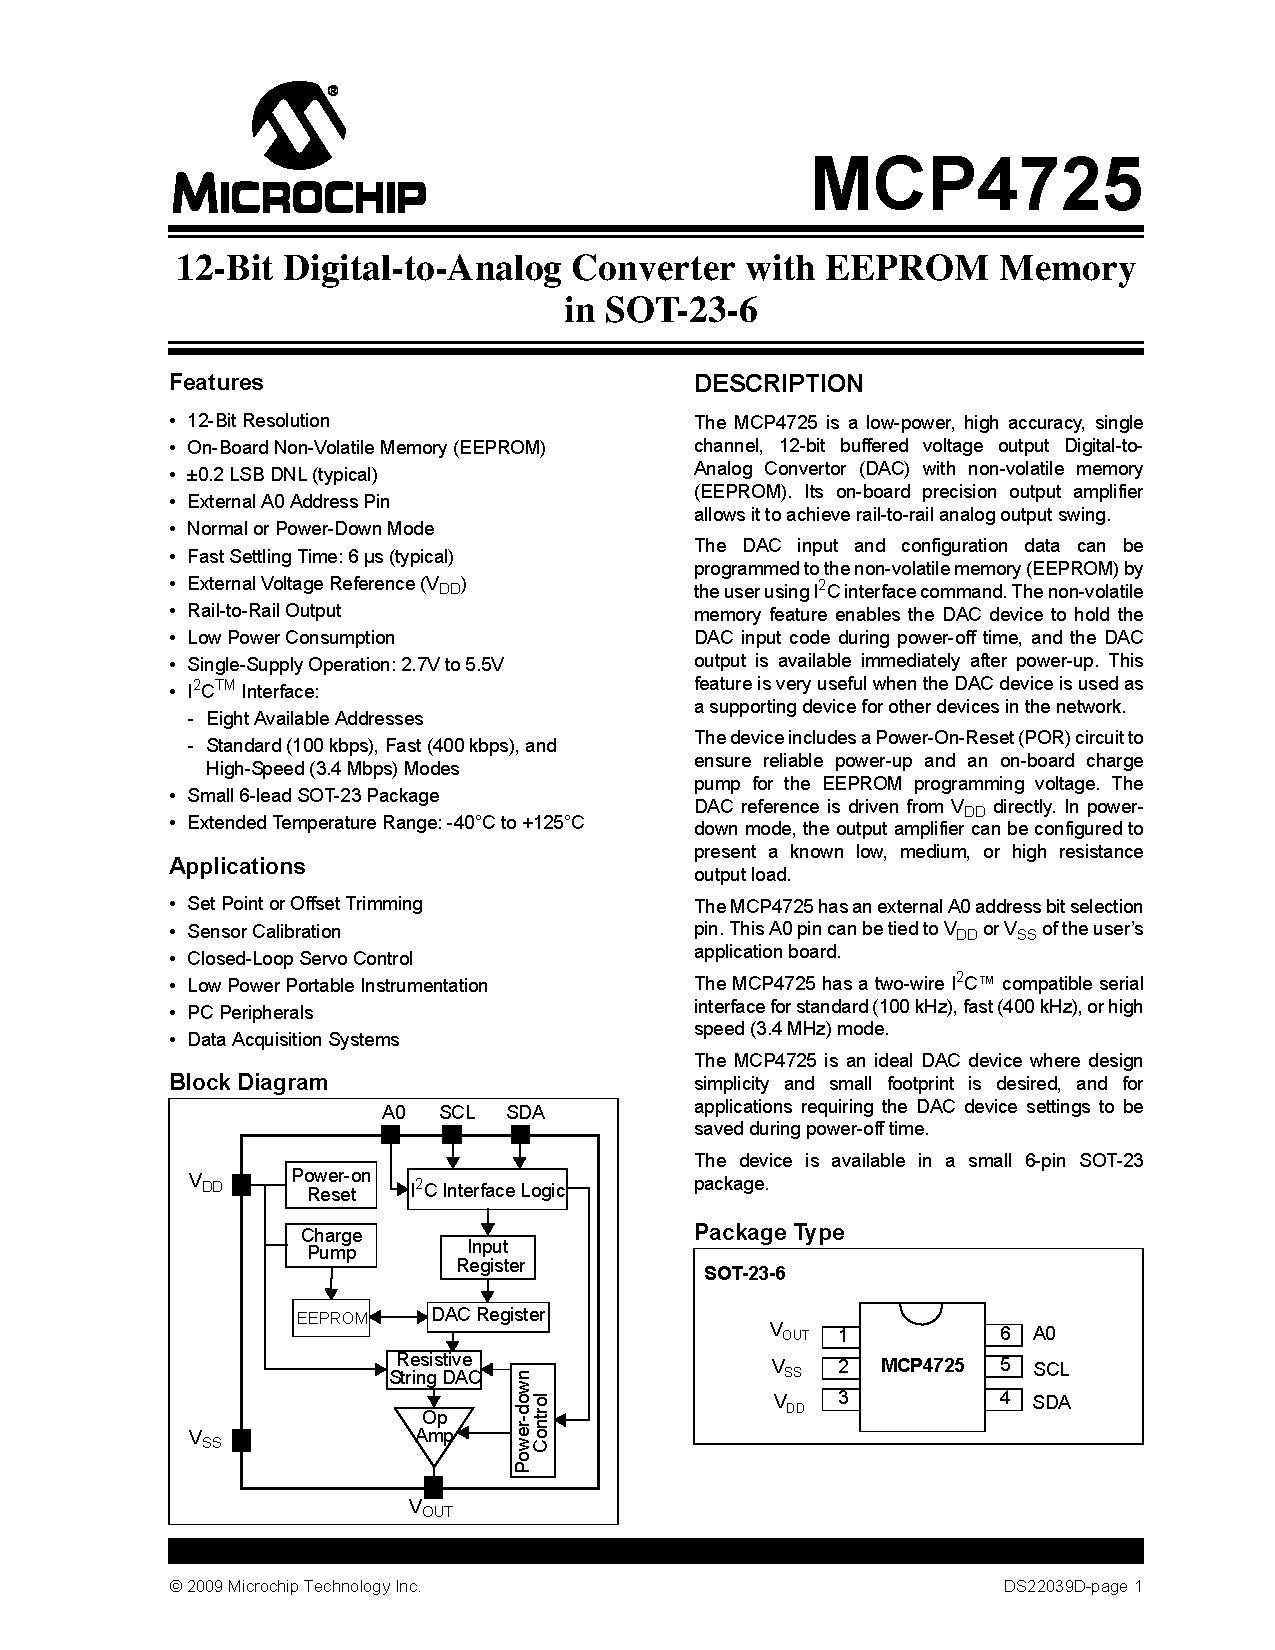
\includepdf[pages={1,3-5,13,15-17}]{./datasheets/mcp4725.pdf} \label{datasheet:mcp4725}

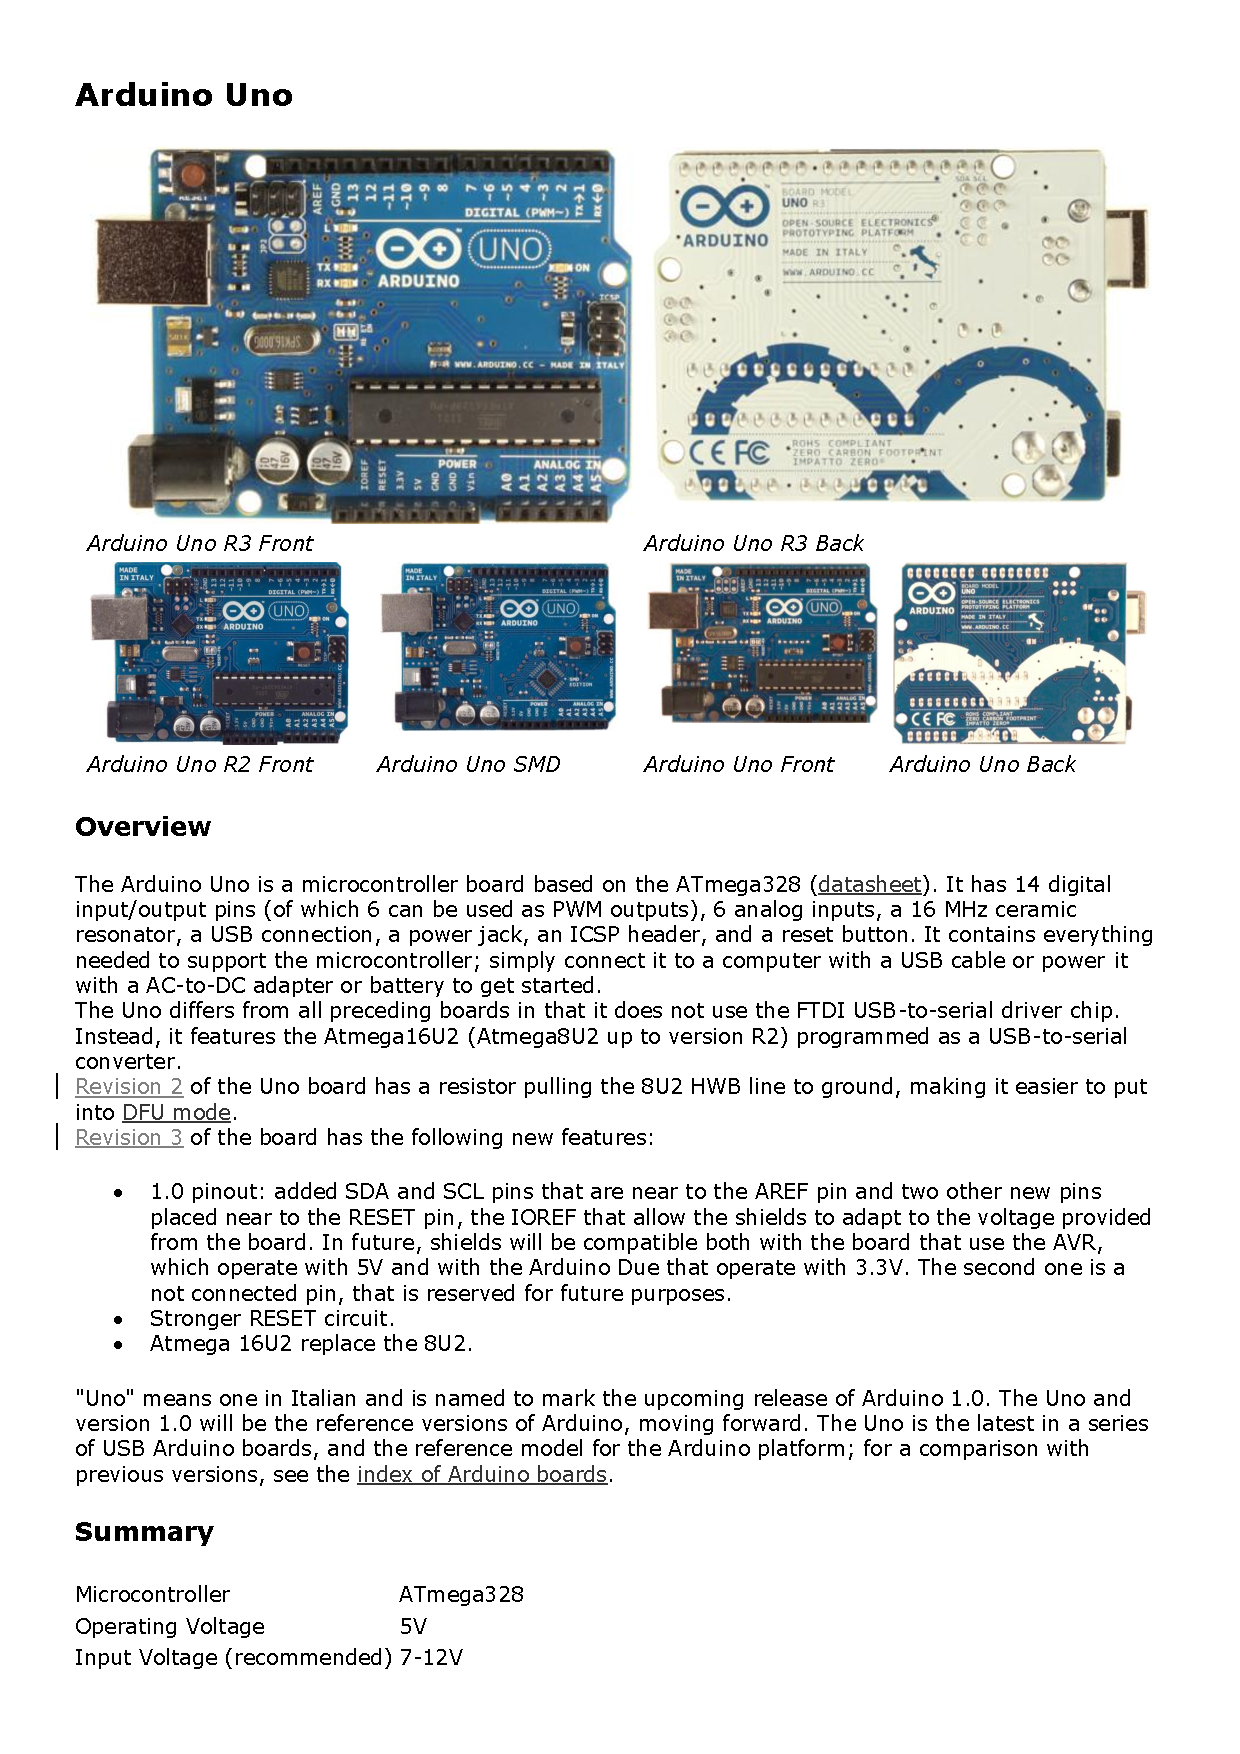
\includepdf[pages=-]{./datasheets/arduino_uno.pdf} \label{datasheet:arduino_uno}

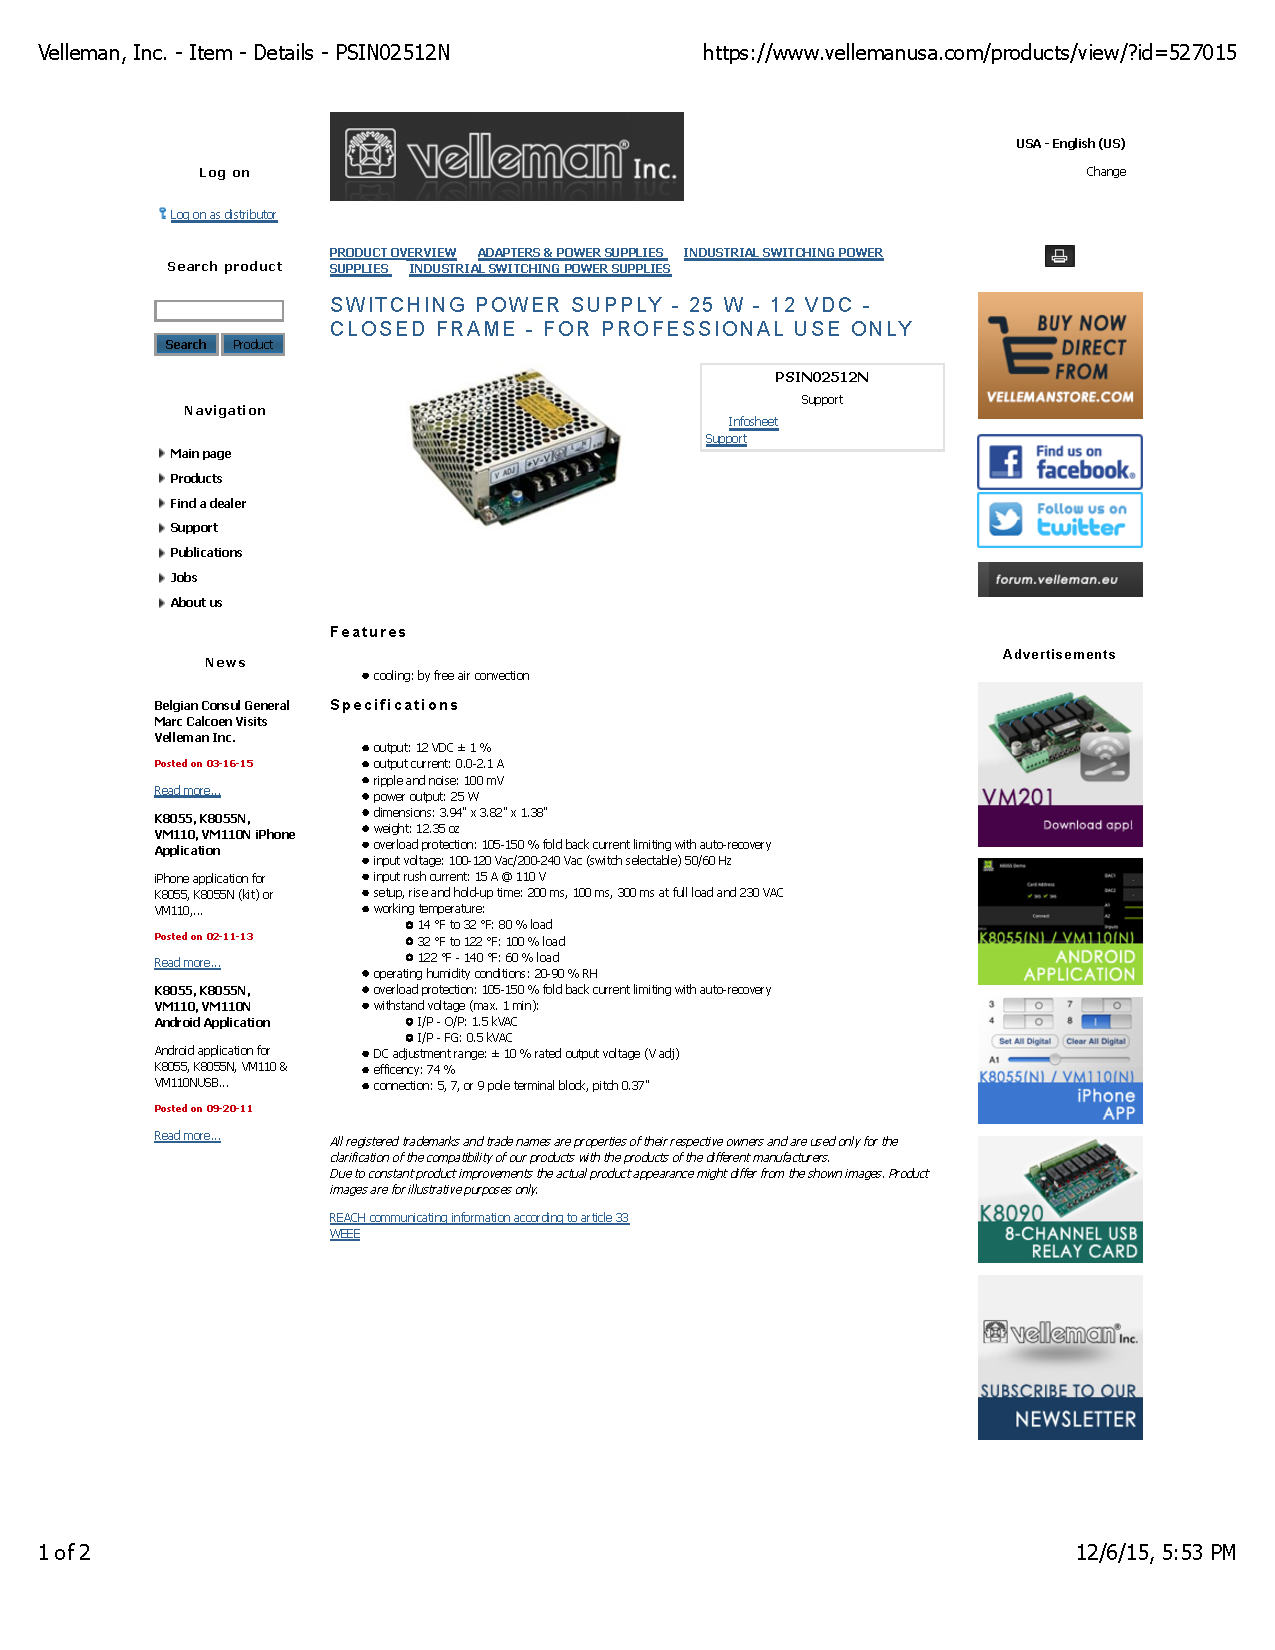
\includepdf[pages=-]{./datasheets/PSIN02512N.pdf} \label{datasheet:psin02512n}

\end{appendices}

\end{document}
